\documentclass[]{beamer}
% Class options include: notes, notesonly, handout, trans,
%                        hidesubsections, shadesubsections,
%                        inrow, blue, red, grey, brown

% Theme for beamer presentation.
\usepackage{beamerthemesplit} 



% Other themes include: beamerthemebars, beamerthemelined, 
%                       beamerthemetree, beamerthemetreebars  

\title{PHY250}    % Enter your title between curly braces
\author{Anabela R. Turlione}                 % Enter your name between curly braces
\institute{Digipen}      % Enter your institute name between curly braces
\date{Fall 2020}                    % Enter the date or \today between curly braces


\begin{document}

% Creates title page of slide show using above information
\begin{frame}
  \titlepage
\end{frame}
%\note{Talk for 30 minutes} % Add notes to yourself that will be displayed when
                           % typeset with the notes or notesonly class options

\section[]{}

% Creates table of contents slide incorporating
% all \section and \subsection commands
\begin{frame}
  \tableofcontents
\end{frame}

%%%%%%%%%%%%%%%%%%%%%%%%%%%%%%%%%%%%%%%%%%%%%%%%%%%%%%%%%%%%%%%%%%%
\section{Wave Motion}

\begin{frame}
\frametitle{Itroduction}

So far we have studied the Simple Harmonic Motion of a single particle...

\begin{center}
  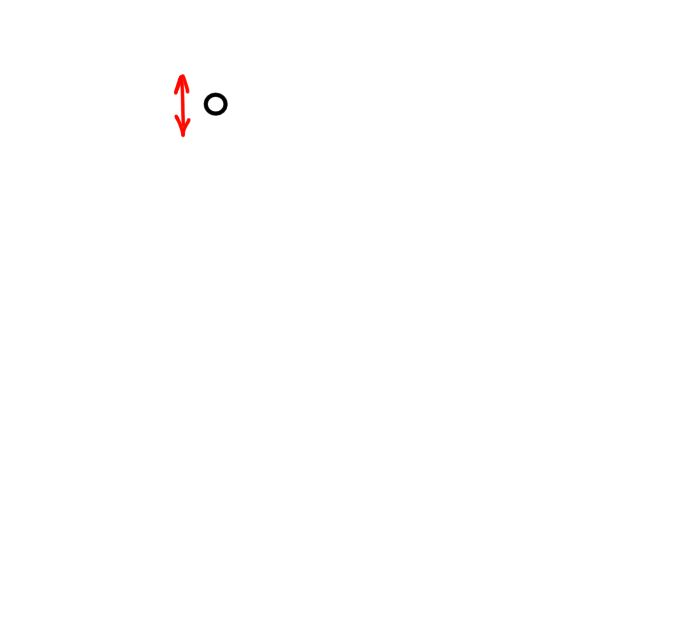
\includegraphics[height=2.2in]{images4/0b.jpg}
\end{center}

  \end{frame}

%%%%%%%%%%%%%%%%%%%%%%%%%%%%%%%%%%%%%%%%%%%%%%%%%%%%%%%%%%%%%%%%%%%


\begin{frame}
\frametitle{Itroduction}

What happens if the the particle that is oscillating is part of a medium? 

\begin{center}
  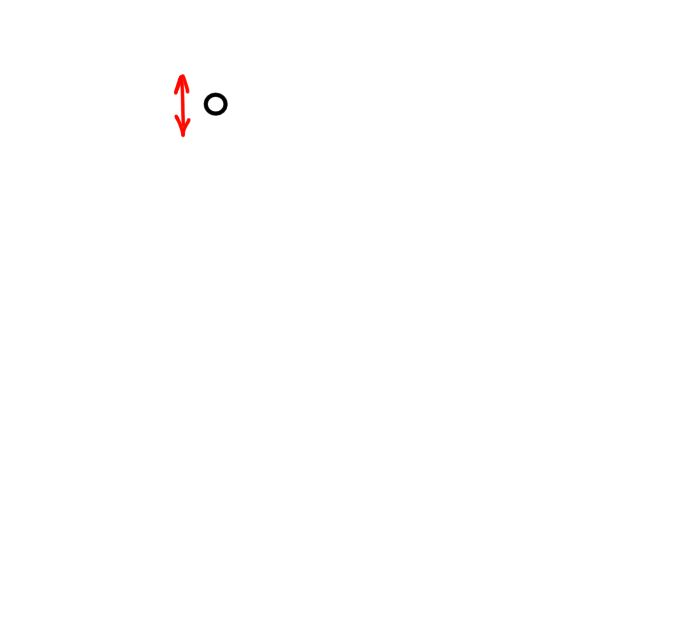
\includegraphics[height=2.2in]{images4/0b.jpg}
\end{center}

  \end{frame}
%%%%%%%%%%%%%%%%%%%%%%%%%%%%%%%%%%%%%%%%%%%%%%%%%%%%%%%%%%%%%%%%%%%


\begin{frame}
\frametitle{Itroduction}

What happens if the the particle that is oscillating is part of a medium? 

\begin{center}
  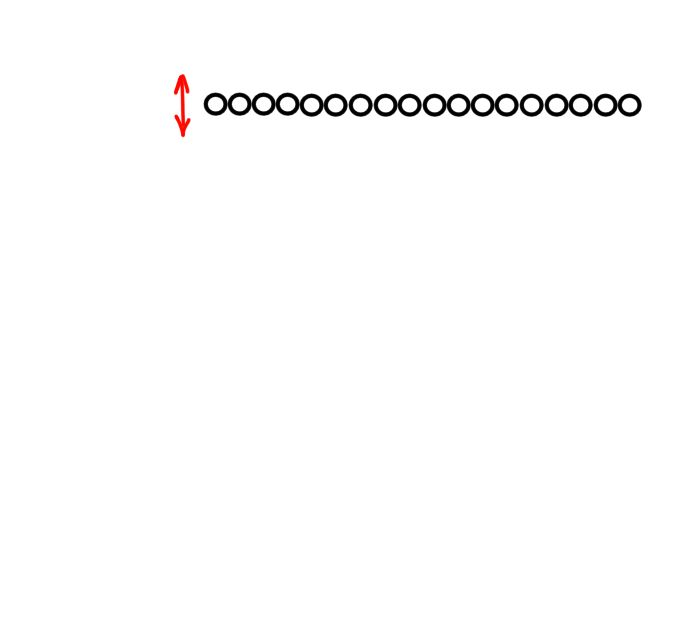
\includegraphics[height=2.2in]{images4/0c.jpg}
\end{center}

  \end{frame}

%%%%%%%%%%%%%%%%%%%%%%%%%%%%%%%%%%%%%%%%%%%%%%%%%%%%%%%%%%%%%%%%%%%
\begin{frame}
\frametitle{Itroduction}

What happens if the the particle that is oscillating is part of a medium? 

\begin{center}
  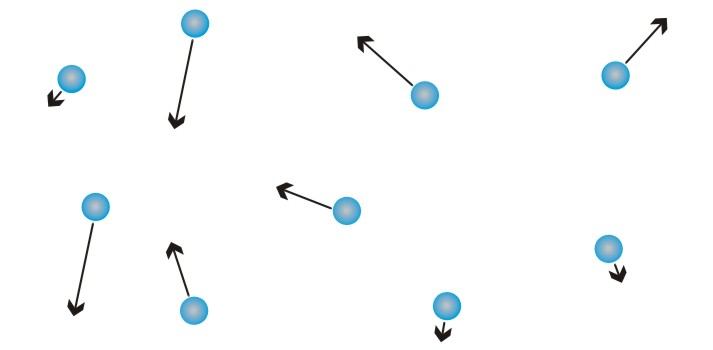
\includegraphics[height=2.2in]{images4/0.jpg}
\end{center}

  \end{frame}

%%%%%%%%%%%%%%%%%%%%%%%%%%%%%%%%%%%%%%%%%%%%%%%%%%%%%%%%%%%%%%%%%%%
\subsection{Characteristic of Wave Motion}

\begin{frame}
\frametitle{Mechanical Waves}

A wave consists of oscillations that moves without carrying matter with them. Examples:
\vspace{3mm}

\pause

\begin{itemize}
\item Sound waves
\pause
\item Waves on a cord
\pause
\item Water waves
\end{itemize}
\vspace{3mm}
\pause
In all those examples, the waves move with a recognizable velocity, but each particle itself merely oscillates about an equilibrium position. Waves can move over large distances, 
but the medium  itself has only a limited motion. 

\vspace{3mm}
\pause
Mechanical Waves carry  Energy as oscillation of matter, they does not carry matter.

\vspace{3mm}

  \end{frame}
%%%%%%%%%%%%%%%%%%%%%%%%%%%%%%%%%%%%%%%%%%%%%%%%%%%%%%%%%%%%%%%%%%%

\begin{frame}
\frametitle{Mechanical Waves}

Example: How a wave is formed in a cord?
\vspace{5mm}

\pause


   \begin{columns}[c]
   \column{2in}  % slides are 3in high by 5in wide
  
\begin{center}
  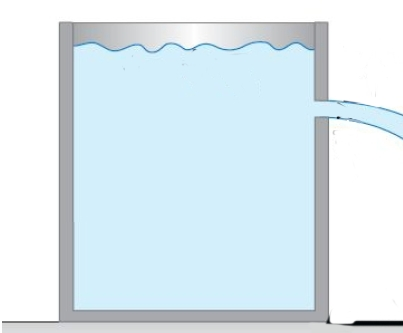
\includegraphics[height=1.7in]{images4/1.jpg}
\end{center}
\pause
   \column{2in}
Single pulse formation: The hand pulls up and down on one end of the cord, each section of the cord is pulled up and down by the tension made by the adjacent section.
The source of the traveling wave pulse is a disturbance, and cohesive forces between adjecent section of the cord cause the pulse to travel.
   \end{columns}






  \end{frame}
%%%%%%%%%%%%%%%%%%%%%%%%%%%%%%%%%%%%%%%%%%%%%%%%%%%%%%%%%%%%%%%%%%%
\begin{frame}
\frametitle{Mechanical Waves}


Source vibrates sinusoidally in a SHM $\rightarrow$ The wave itself will have a sinusoidal shape that depends on both,  time and space. 
\pause
\vspace{5mm}

\begin{enumerate}
\item In space: If you take a picture of the wave in a given instant of time, the wave will have the shape of a sine or a cosine.
\pause
\item In time: the up-down motion of  an small segment  of  the cord at a certain position will be Simple Harmonic Motion.

\end{enumerate}

  \end{frame}

%%%%%%%%%%%%%%%%%%%%%%%%%%%%%%%%%%%%%%%%%%%%%%%%%%%%%%%%%%%%%%%%%%%
\begin{frame}
\frametitle{Periodic Sinusoidal Waves}



Picture of the wave at a certain time:
\pause

\vspace{5mm}

  \begin{center}
  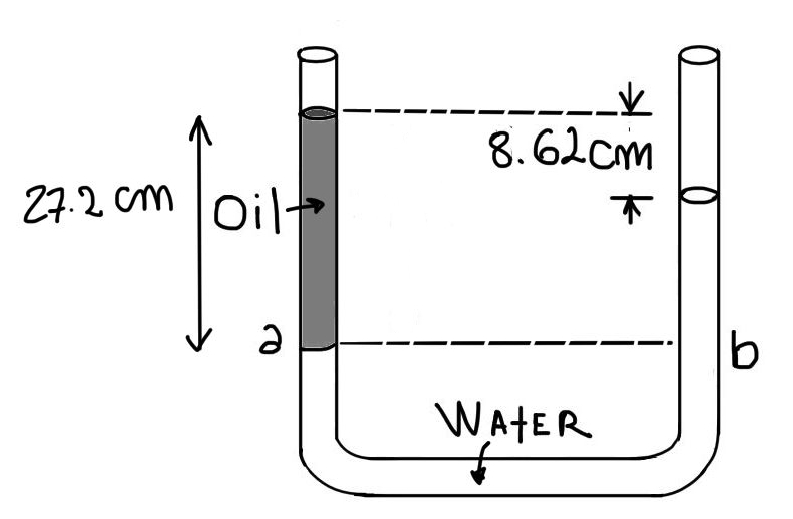
\includegraphics[height=1.5in]{images4/2.jpg}
\end{center}
\pause
The \textbf{wave velocity}, $v$, is the velocity at which wave crests move forward. 
\pause
\begin{equation}
v=\lambda /T=\lambda f
\end{equation}

  \end{frame}

%%%%%%%%%%%%%%%%%%%%%%%%%%%%%%%%%%%%%%%%%%%%%%%%%%%%%%%%%%%%%%%%%%%
\begin{frame}
\frametitle{Types of waves}
\pause
 \begin{itemize}
\item \textbf{Transverse waves} The vibration up-down  of the particles of the medium are in a direction transverse to the motion of the wave itself.
\pause
\item \textbf{Logitudinal Waves} The vibration of the particles in the medium is along the direction of the wave's motion.
\pause
\end{itemize}

\pause

 \begin{center}
  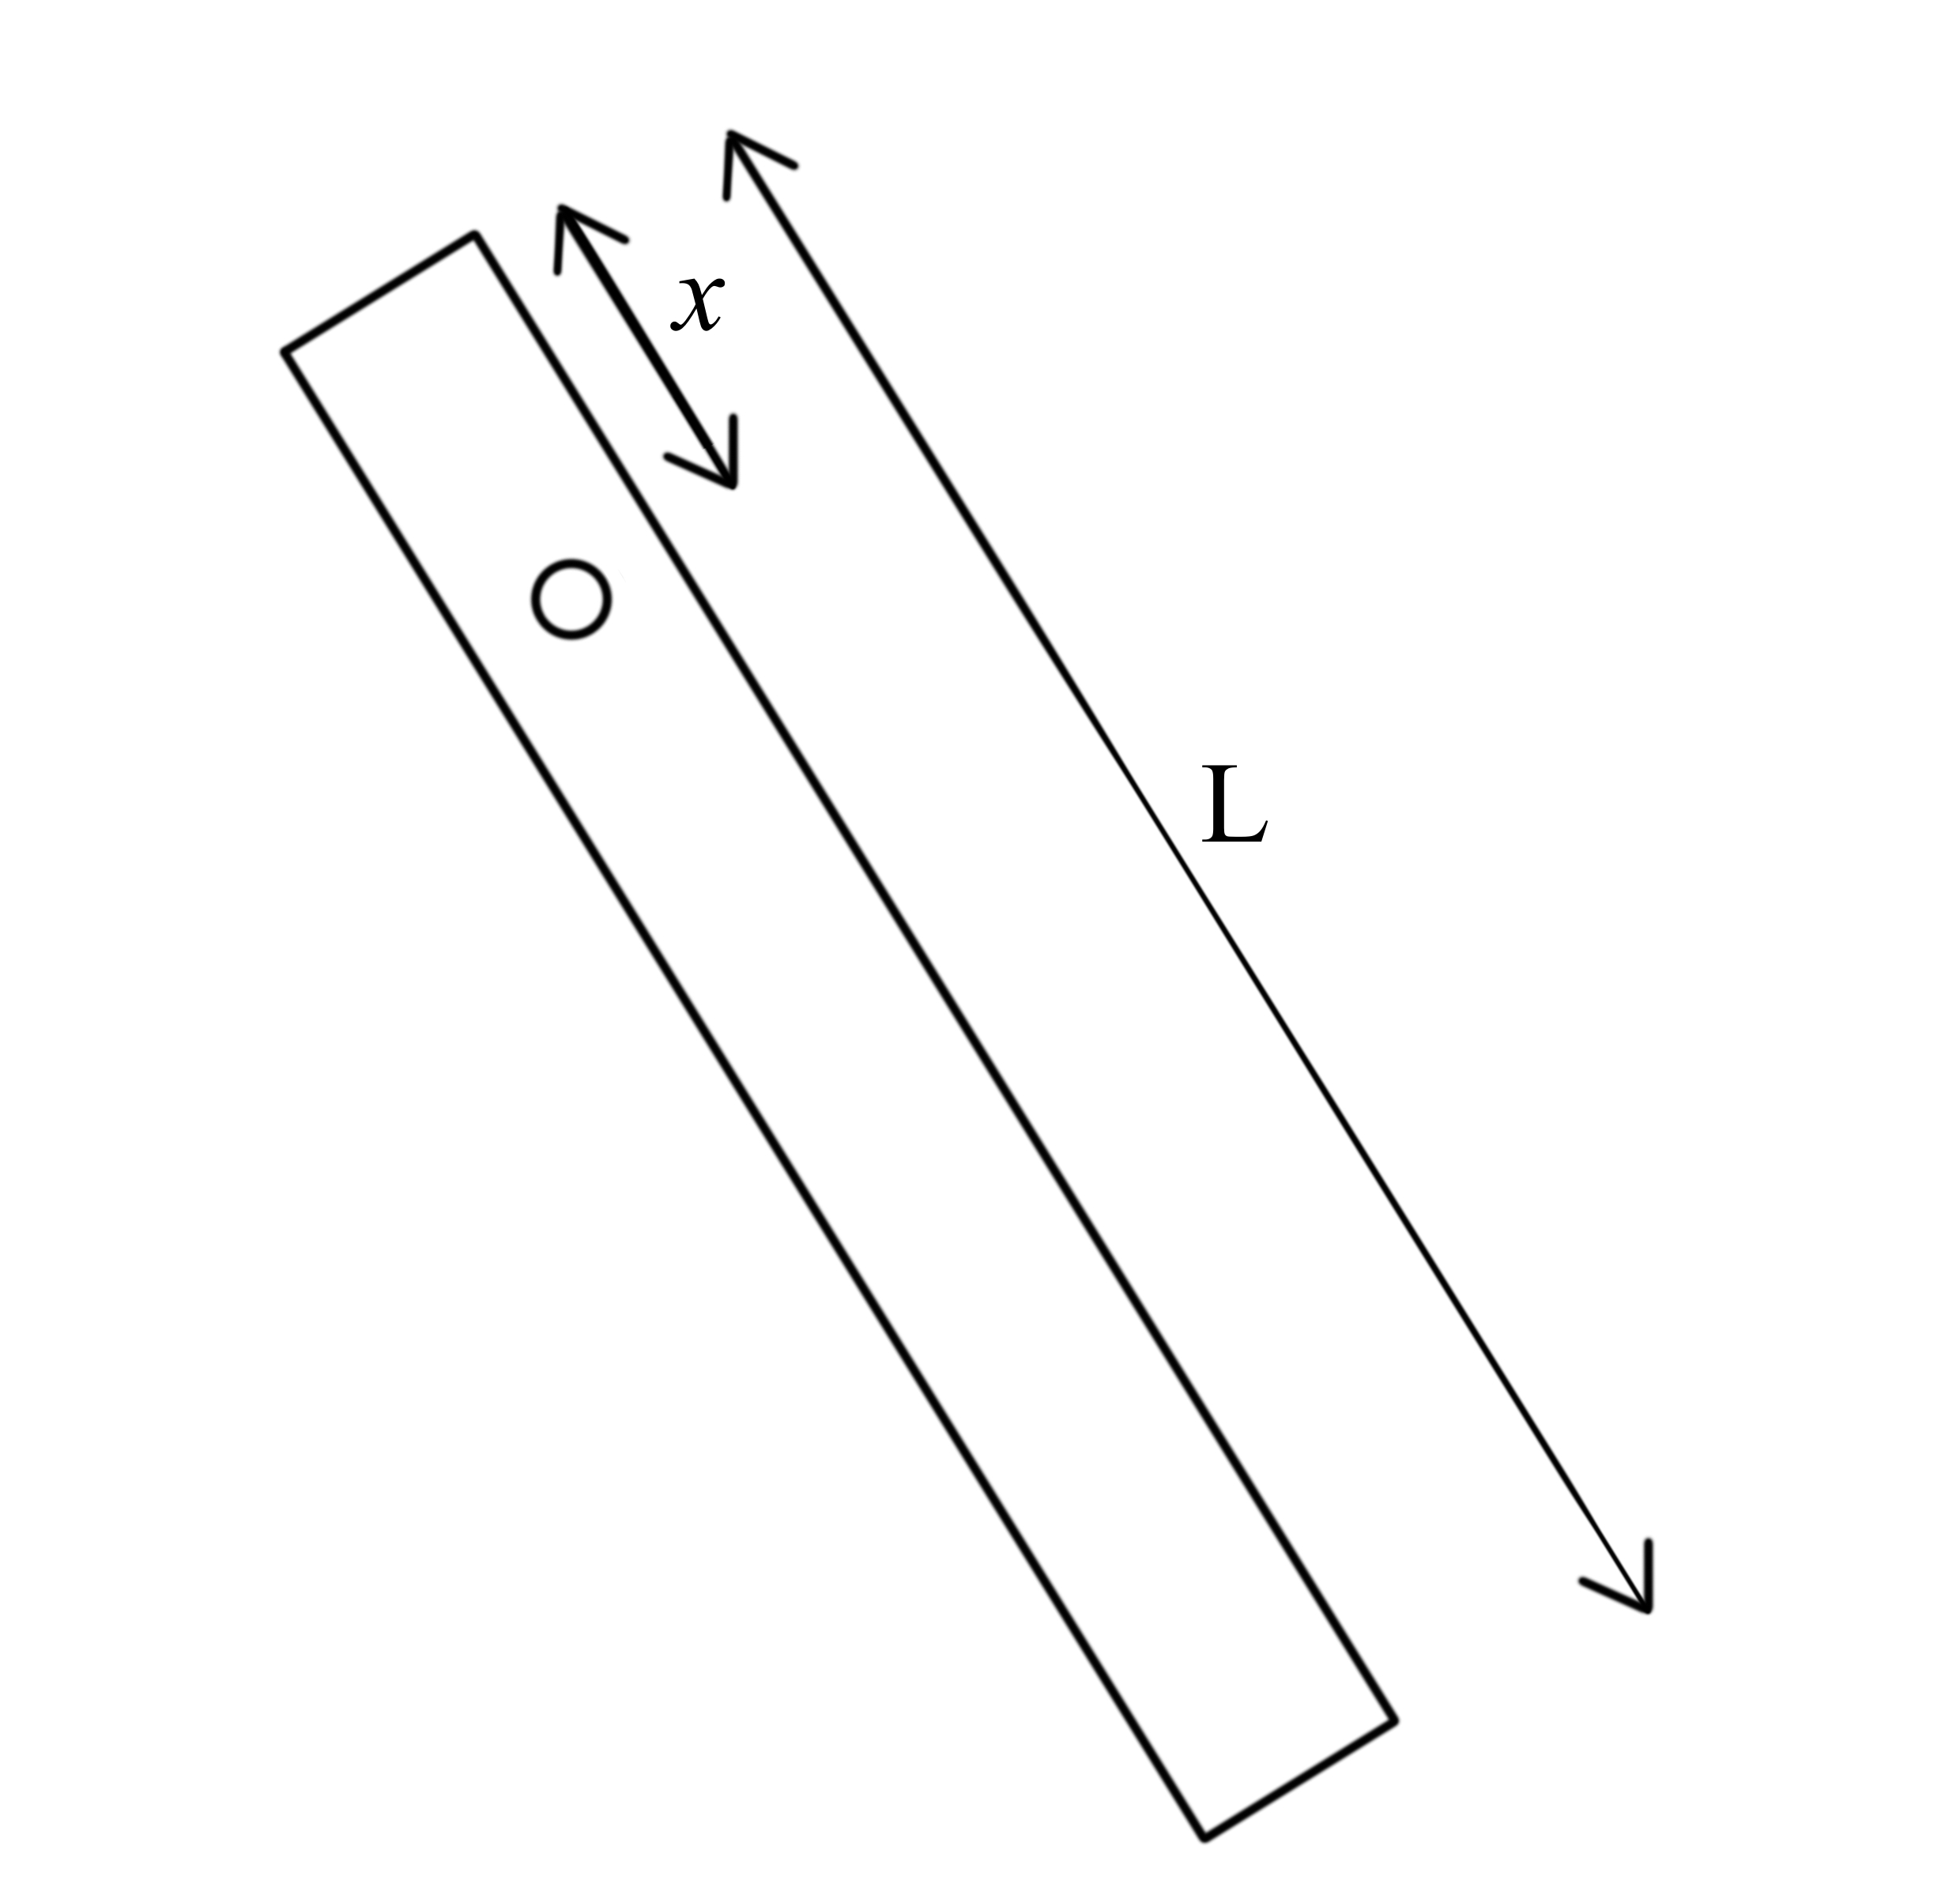
\includegraphics[height=1.5in]{images4/3.jpg}
\end{center}

  \end{frame}




%%%%%%%%%%%%%%%%%%%%%%%%%%%%%%%%%%%%%%%%%%%%%%%%%%%%%%%%%%%%%%%%%%%
\begin{frame}
\frametitle{Types of waves}

Sound waves: example of longitidinal waves.
\pause

\vspace{5mm}

 A vibrating drumhead, for instance, alternately compresses and rarefies the air in contact with it,
producing a longitudinal wave that travels outward in the air. 
\pause
 \begin{center}
  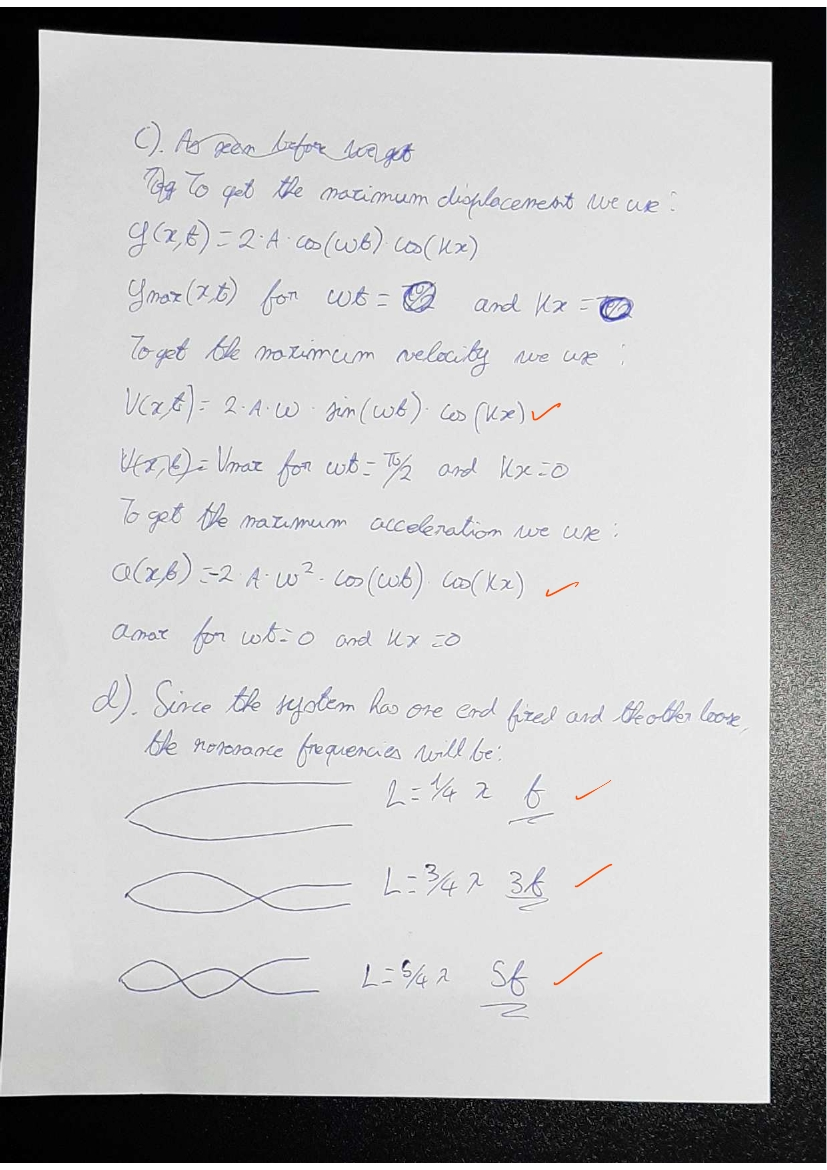
\includegraphics[height=1.5in]{images4/5.jpg}
\end{center}

  \end{frame}


%%%%%%%%%%%%%%%%%%%%%%%%%%%%%%%%%%%%%%%%%%%%%%%%%%%%%%%%%%%%%%%%%%%
\begin{frame}
\frametitle{Types of waves}

A longitudinal wave can be represented graphically by plotting the density of
air molecules versus position at a given instant.
\pause

 \begin{center}
  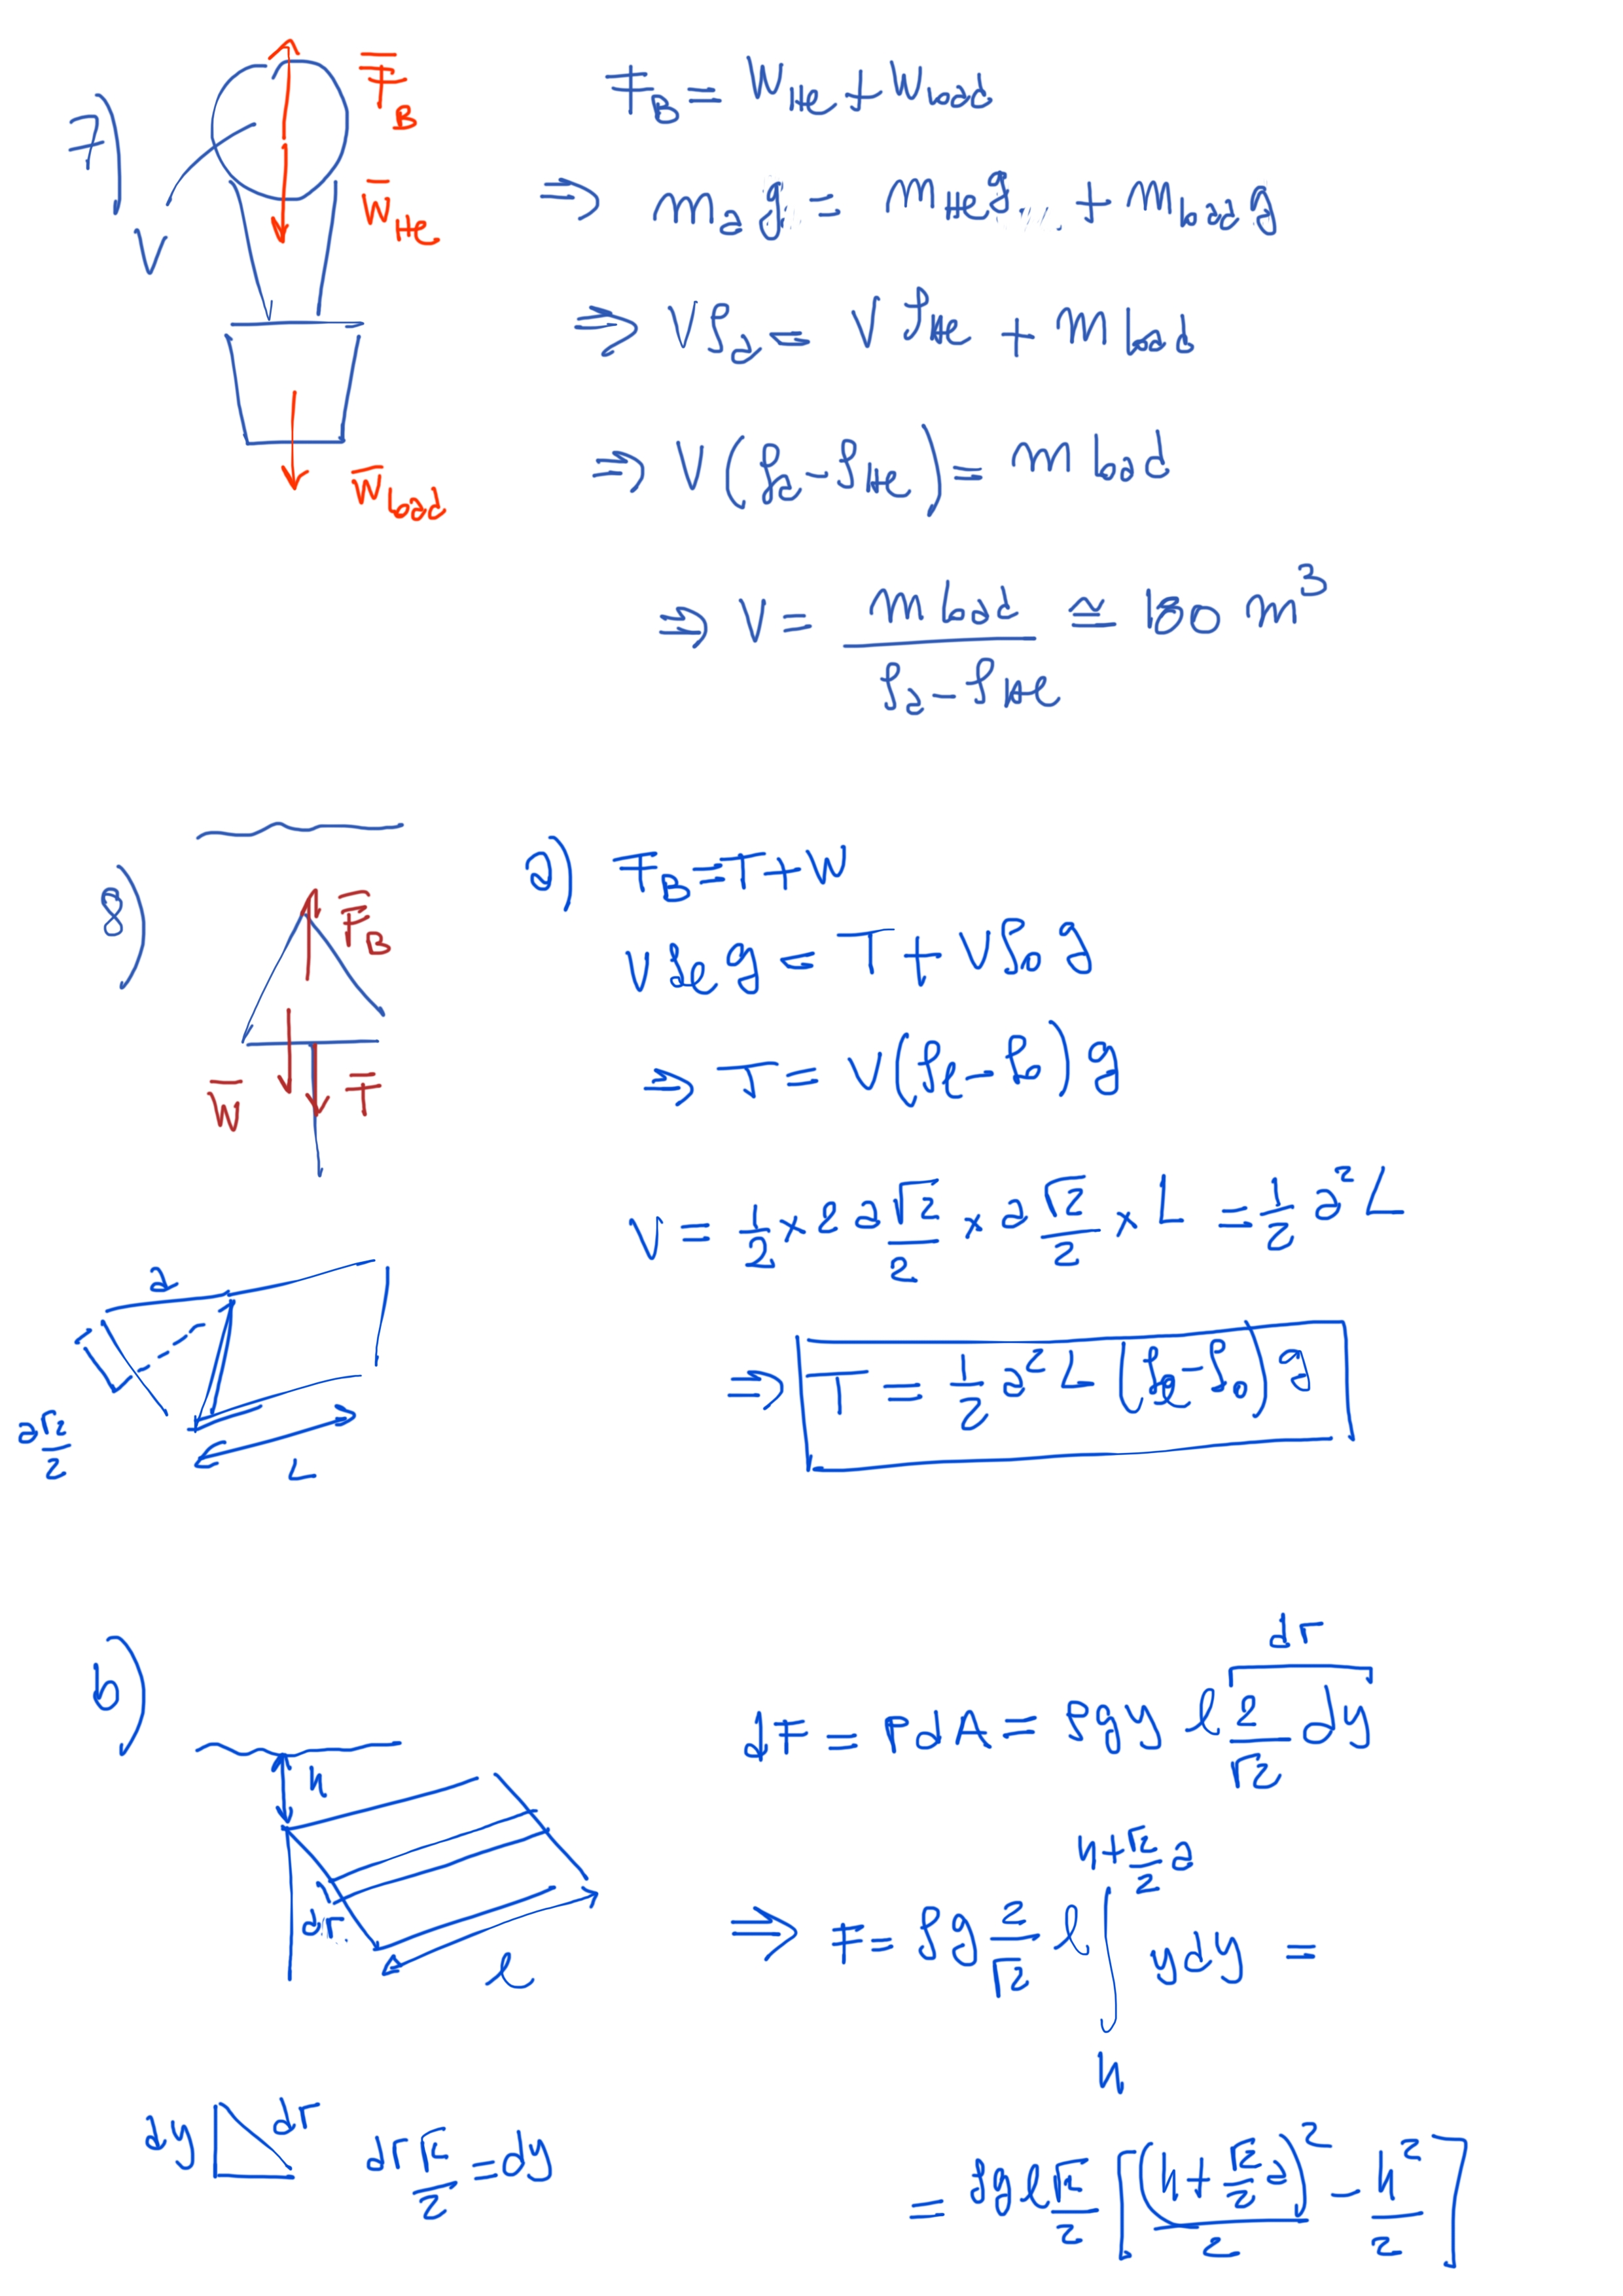
\includegraphics[height=1.5in]{images4/4.jpg}
\end{center}

  \end{frame}



%%%%%%%%%%%%%%%%%%%%%%%%%%%%%%%%%%%%%%%%%%%%%%%%%%%%%%%%%%%%%%%%%%%
\begin{frame}
\frametitle{Velocity of transverse Waves}
The velocity of a wave depends on the properties of the medium in which it travels.
\pause

\begin{equation}
v=\sqrt{\frac{F_T}{\mu}}
\end{equation}
\pause

where, $F_T$ is the tension on the cord and $\lambda$ is the longitudinal density.


  \end{frame}

%%%%%%%%%%%%%%%%%%%%%%%%%%%%%%%%%%%%%%%%%%%%%%%%%%%%%%%%%%%%%%%%%%%
\begin{frame}
\frametitle{Velocity of transverse Waves}
Proof:




   \begin{columns}[c]
   \column{2.5in}  % slides are 3in high by 5in wide

 \begin{center}
  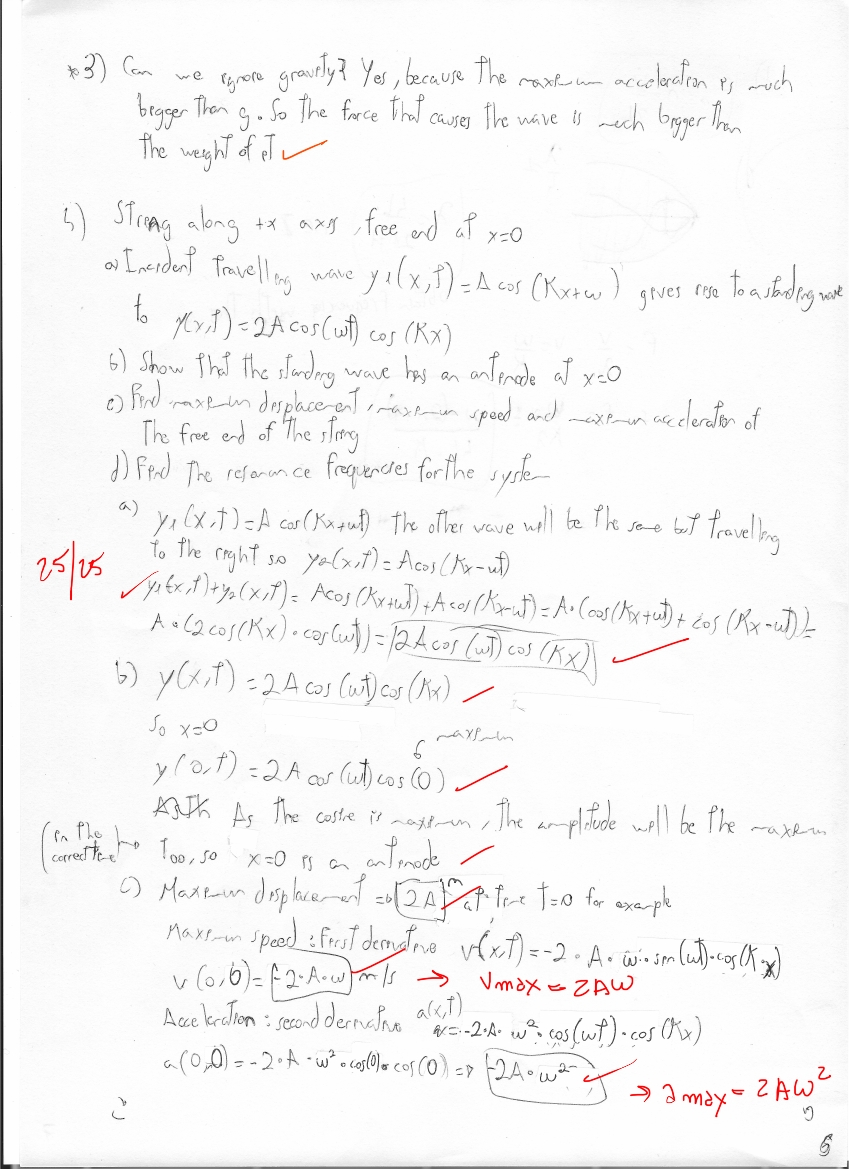
\includegraphics[height=1.5in]{images4/6.jpg}
\end{center}

  \pause
Small vertical displacement ($v't\ll vt$)
\pause
\begin{equation}
\frac{F_y}{F_T}=\frac{v't}{vt}=\frac{v'}{v}
\end{equation}
\pause
   \column{2.in}

Impulse:

 \begin{equation*}
F_y t=\Delta P'=\Delta mv'
\end{equation*}
\pause
\begin{equation*}
\Delta m=\mu x=\mu vt
\end{equation*}
\pause
\begin{equation*}
\rightarrow F_y t=\mu vtv' \rightarrow \frac{v'}{v}F_T=\mu vv'
\end{equation*}
\pause

\begin{equation}
\rightarrow v=\sqrt{\frac{F_T}{\mu}}
\end{equation}

   \end{columns}



  \end{frame}



%%%%%%%%%%%%%%%%%%%%%%%%%%%%%%%%%%%%%%%%%%%%%%%%%%%%%%%%%%%%%%%

\begin{frame}
\frametitle{Velocity of transverse Waves}

In general...

\pause
\begin{equation*}
 v=\sqrt{\frac{elastic~force~factor}{inertia~factor}}
\end{equation*}
\pause
\vspace{2mm}

Longitudinal wave traveling down a long solid rod $ \rightarrow v=\sqrt{\frac{E}{\rho}}$

\pause
\vspace{2mm}
Longitudinal wave traveling in a liquid or gas $ \rightarrow v=\sqrt{\frac{B}{\rho}}$

\pause
\vspace{4mm}
Where, $E$ and $B$ are the elastic and bulk modulus, respectively.

  \end{frame}


%%%%%%%%%%%%%%%%%%%%%%%%%%%%%%%%%%%%%%%%%%%%%%%%%%%%%%%%%%%%%%%
\subsection{Energy transported by a wave}
\begin{frame}

Waves transport energy from one place to another. For a sinusoidal wave of frequency $f$ , the particles move in
simple harmonic motion.
\pause
\vspace{2mm}

As a wave passes, each particle has an energy
\pause

\begin{equation}
 E=\frac{1}{2} k A^2=\frac{1}{2} \omega^2 mA^2= 2\pi^2 mf^2A^2
\end{equation}

\pause
For three-dimensional waves traveling in an elastic medium, $m=\rho V$, and $V=S\ell$ and $\ell=vt$ (see the figure):

\pause
  \begin{center}
  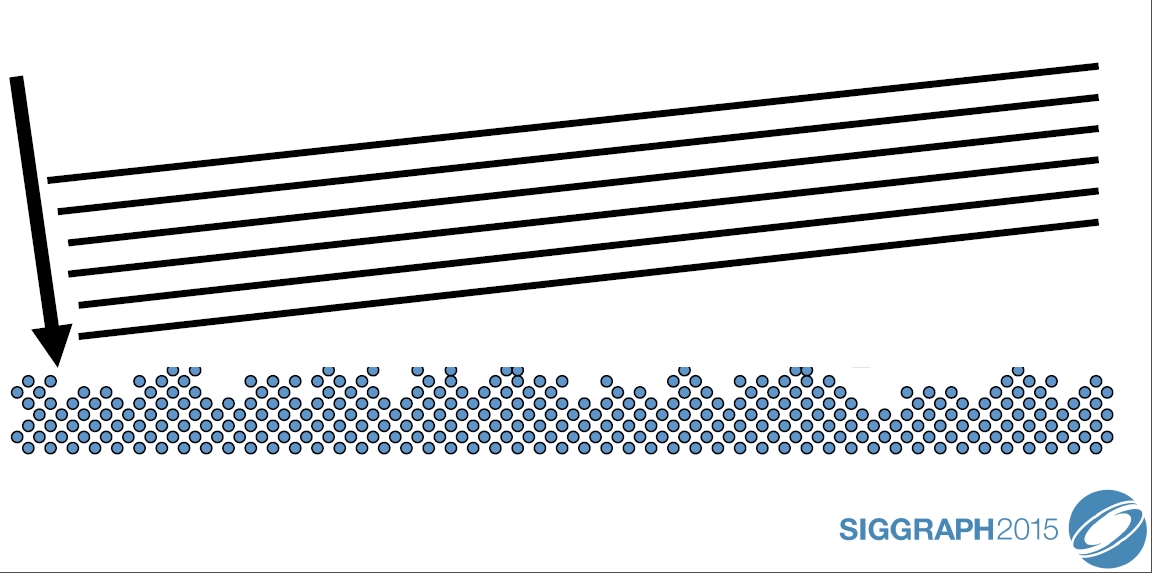
\includegraphics[height=1.4in]{images4/7.jpg}
\end{center}


  \end{frame}

%%%%%%%%%%%%%%%%%%%%%%%%%%%%%%%%%%%%%%%%%%%%%%%%%%%%%%%%%%%%%%%

\begin{frame}
Then, the energy is

\begin{equation}
E=2\pi^2\rho S v t f^2A^2
\end{equation}

\textit{The energy transported by a
wave is proportional to the square of the amplitude, and to the square o f the
frequency}.
\vspace{2mm}

\pause

The average rate of energy transferred is the average power P:

\pause

\begin{equation}
\overline P=\frac{E}{t}
\end{equation}


\end{frame}
%%%%%%%%%%%%%%%%%%%%%%%%%%%%%%%%%%%%%%%%%%%%%%%%%%%%%%%%%%%%%%%



\begin{frame}


The \textbf{ intensity}, $I$, of a wave is defined as the average power transferred
across unit area perpendicular to the direction of energy flow:

\pause

\begin{equation}
I= \frac{\overline P}{S}=\frac{E}{tS}=2\pi^2\rho  v f^2A^2
\end{equation}
\end{frame}
%%%%%%%%%%%%%%%%%%%%%%%%%%%%%%%%%%%%%%%%%%%%%%%%%%%%%%%%%%%%%%%


\begin{frame}
\frametitle{Point source in an isotropic medium}



   \begin{columns}[c]
   \column{2in}  % slides are 3in high by 5in wide
  
\pause

 \begin{center}
  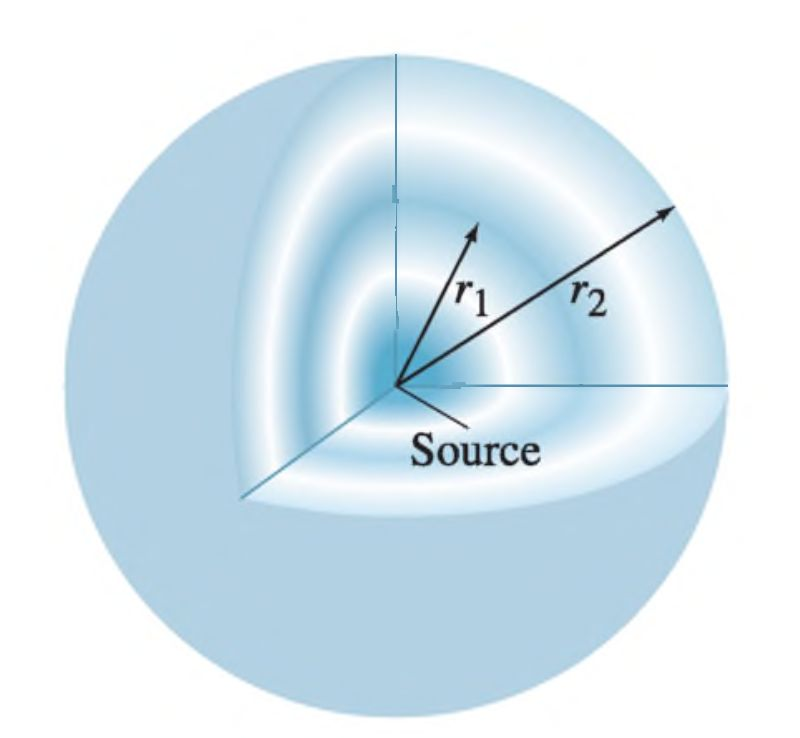
\includegraphics[height=1.2in]{images4/8.jpg}
\end{center}

   \column{2.4in}

\pause


If the medium is isotropic, the wave from a point source is
a spherical wave, the intensity is,

\pause

\begin{equation}
I=\frac{\overline P}{S}=\frac{\overline P}{4\pi r^2}
\end{equation}


   \end{columns}

\pause

If the power output P is constant $\rightarrow I\propto \frac{1}{r^2}$
\vspace{2mm}

\pause

When the distance doubles, then the intensity is
reduced to $1/4$. The amplitude of a wave also decreases with distance,

\pause

\begin{equation}
A\propto \frac{1}{r}
\end{equation}

\pause

wave is twice as far from the source $\rightarrow$ amplitude is half as large.

  \end{frame}

%%%%%%%%%%%%%%%%%%%%%%%%%%%%%%%%%%%%%%%%%%%%%%%%%%%%%%%%%%%%%%%
\subsection{Mathematical description of a Wave}

\begin{frame}
\pause

Suppose that at $t=0$, the wave shape is,

\pause
\begin{equation}
D(x)=Asin\frac{2\pi}{\lambda}x
\end{equation}

\pause

where $D(x)$ is the displacement of the wave at point x. If the wave is moving to the right, with velocity $v$, then,

\pause

\begin{equation}
D(x,t)=Asin\frac{2\pi}{\lambda}(x-vt)
\end{equation}

\pause

 \begin{center}
  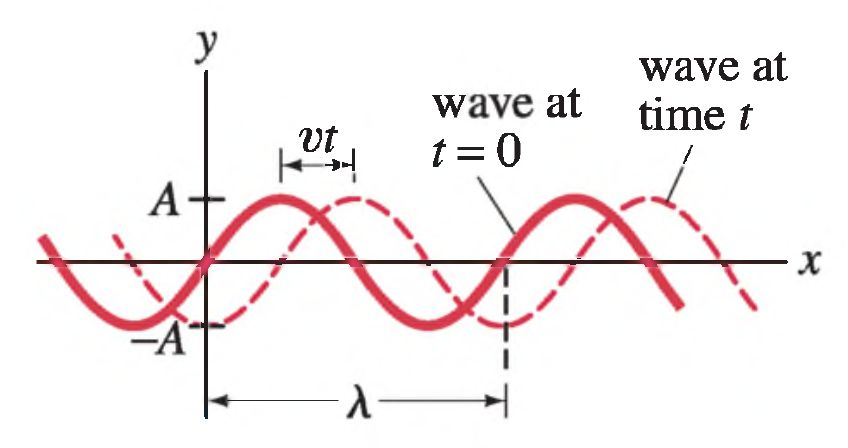
\includegraphics[height=1.2in]{images4/9.jpg}
\end{center}



  \end{frame}

%%%%%%%%%%%%%%%%%%%%%%%%%%%%%%%%%%%%%%%%%%%%%%%%%%%%%%%%%%%%%%%
\begin{frame}


We can writethe expression ofr $D(x,t) $as,

\pause

\begin{equation}
D(x,t)=Asin(\frac{2\pi}{\lambda}x-\frac{2\pi}{\lambda}vt)=Asin(\frac{2\pi}{\lambda}x-\frac{2\pi}{T}t)
\end{equation}

\pause

where $v=\frac{\lambda}{T}$.

\pause

Then,

\pause

\begin{equation}
D(x,t)=Asin(kx-\omega t)
\end{equation}

\pause


where $k=\frac{2\pi}{\lambda}$ is called the \textbf{wave number}. The quantity $(kx-\omega t)$ is called the phase of the wave, and $v$ is the phase velocity.

\pause
\begin{equation}
v=\frac{2\pi}{k}\frac{\omega}{2\pi}=\frac{\omega}{k}
\end{equation}

  \end{frame}


%%%%%%%%%%%%%%%%%%%%%%%%%%%%%%%%%%%%%%%%%%%%%%%%%%%%%%%%%%%%%%%
\begin{frame}


Wave traveling to the left:

\pause

\begin{equation}
D(x,t)=Asin(kx+\omega t)
\end{equation}

\pause

The argument of the sine can also contain a phase $\phi$ determined by the value of $D$ at $x=0,~t=0$.
  \end{frame}


%%%%%%%%%%%%%%%%%%%%%%%%%%%%%%%%%%%%%%%%%%%%%%%%%%%%%%%%%%%%%%%
\subsection{The Wave Equation}

\begin{frame}


\frametitle{The Wave Equation}






Many types of waves satisfy an important general equation that is the equivalent
of Newton’s second law of motion for particles.

\pause

We assume:

\pause

\begin{itemize}
\item The amplitude of the wave is small compared to the wavelength.

\pause
\item The tension in the string does not vary during a vibration.
\end{itemize}


  \end{frame}




%%%%%%%%%%%%%%%%%%%%%%%%%%%%%%%%%%%%%%%%%%%%%%%%%%%%%%%%%%%%%%%


\begin{frame}
\frametitle{The Wave Equation}



   \begin{columns}[c]
   \column{2in}  % slides are 3in high by 5in wide
   \begin{center}
  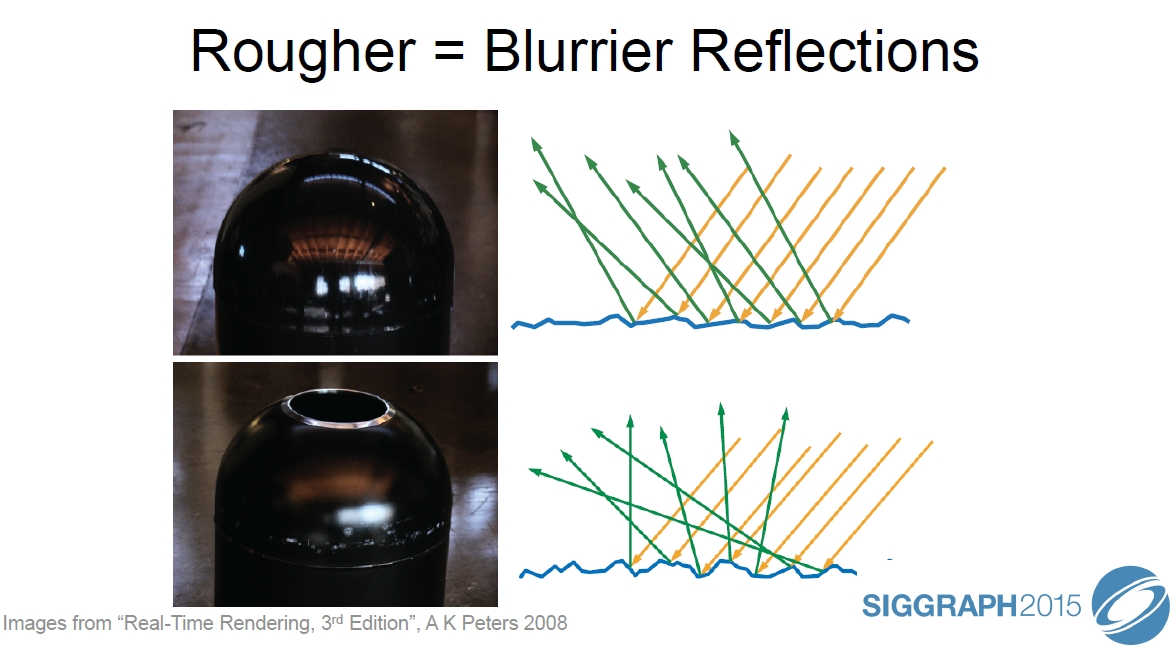
\includegraphics[height=1.in]{images4/10.jpg}
\end{center}




\begin{equation*}
\sum F_y=ma_y
\end{equation*}

\pause

   \column{2.5in}

\begin{equation*}
F_Tsin\theta_2-F_Tsin\theta_1=(\mu\Delta x)\frac{\partial^2 D}{\partial t^2}
\end{equation*}

\pause

where, $a_y=\frac{\partial^2 D}{\partial t^2}$ because the motion is vertical.


\pause

The angles are small, then

\pause

\begin{equation*}
sin\theta\approx tan\theta=\frac{\partial D}{\partial x}=S
\end{equation*}

\pause




   \end{columns}









  \end{frame}







%%%%%%%%%%%%%%%%%%%%%%%%%%%%%%%%%%%%%%%%%%%%%%%%%%%%%%%%%%%%%%%


\begin{frame}
\frametitle{The Wave Equation}


Then, our equation becomes,

\pause

\begin{equation}
F_T(S_2-S_1)=\mu \Delta x\frac{\partial^2D}{\partial^2 t}
\end{equation}

Or..

\pause

\begin{equation}
F_T\frac{\Delta S}{\Delta x}=\mu \frac{\partial^2D}{\partial^2 t}
\end{equation}

\pause

now we take the limit of $\Delta x \rightarrow 0$, so that
\pause

\begin{equation}
\lim_{x\to 0} F_T\frac{\Delta S}{\Delta x}=F_T\frac{\partial}{\partial x}\left(\frac{\partial D}{\partial x}\right)=F_T\frac{\partial^2D}{\partial x^2}
\end{equation}
\pause




  \end{frame}






%%%%%%%%%%%%%%%%%%%%%%%%%%%%%%%%%%%%%%%%%%%%%%%%%%%%%%%%%%%%%%%


\begin{frame}
\frametitle{The Wave Equation}

Then,

\pause

\begin{equation}
\frac{\partial^2D}{\partial x^2}=\frac{\mu}{F_T} \frac{\partial^2D}{\partial^2 t}
\end{equation}

We saw earlier that 
\pause

\begin{equation*}
\rightarrow v=\sqrt{\frac{F_T}{\mu}}
\end{equation*}


  \end{frame}


%%%%%%%%%%%%%%%%%%%%%%%%%%%%%%%%%%%%%%%%%%%%%%%%%%%%%%%%%%%%%%%


\begin{frame}
\frametitle{The Wave Equation}



Then,


\begin{equation}
\frac{\partial^2D}{\partial x^2}=\frac{1}{v^2} \frac{\partial^2D}{\partial^2 t}
\end{equation}

\pause

This is the \textbf{one-dimensional} wave equation, and it can describe not only small
amplitude waves on a stretched string, but also small amplitude longitudinal waves
 in gases, liquids, and elastic solids..

  \end{frame}

%%%%%%%%%%%%%%%%%%%%%%%%%%%%%%%%%%%%%%%%%%%%%%%%%%%%%%%%%%%%%%%

\section{Superposition Principle}

\begin{frame}
\frametitle{Superposition Principle}

If $D_1$ and $D_2$ are solutions of 

\begin{equation*}
\frac{\partial^2D}{\partial x^2}=\frac{1}{v^2} \frac{\partial^2D}{\partial^2 t}
\end{equation*}

Then, the sum $D_1+D_2$ is also a solution..
\vspace{3mm}

\pause

In general, when two or more waves pass through the same region of space at the same time,
it is found that the displacement is the vector (or algebraic)
sum of the separate displacements.


  \end{frame}





%%%%%%%%%%%%%%%%%%%%%%%%%%%%%%%%%%%%%%%%%%%%%%%%%%%%%%%%%%%%%%%


\begin{frame}
\frametitle{Superposition Principle}



   \begin{columns}[c]
   \column{2in}  % slides are 3in high by 5in wide
  
Example:  In this case
there are three waves present, on a stretched string, each of different amplitude
and frequency.The resultant wave is not a simple sinusoidal wave and is called a composite
(or complex) wave

   \column{2in}


  \begin{center}
  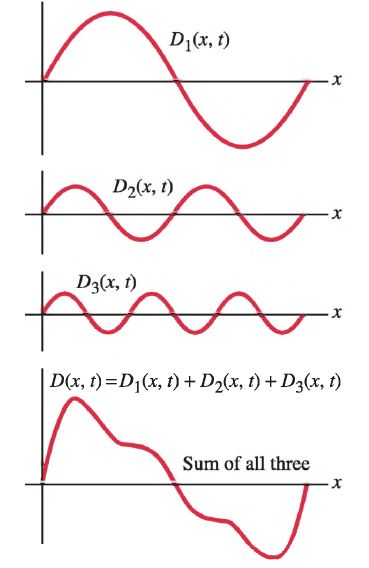
\includegraphics[height=2.5in]{images4/11.jpg}
\end{center}


   \end{columns}




  \end{frame}


%%%%%%%%%%%%%%%%%%%%%%%%%%%%%%%%%%%%%%%%%%%%%%%%%%%%%%%%%%%%%%%


\begin{frame}
\frametitle{Superposition Principle}


It can be shown that any complex wave can be considered as being composed of
many simple sinusoidal waves of different amplitudes, wavelengths, and frequencies.
This is known as Fourier’s theorem. A complex periodic wave of period T can be
represented as a sum of pure sinusoidal terms whose frequencies are integral
multiples of $f = 1/T$.



\vspace{3mm}
If the wave is not periodic, the sum becomes an integral
(called a Fourier integral).


  \end{frame}


%%%%%%%%%%%%%%%%%%%%%%%%%%%%%%%%%%%%%%%%%%%%%%%%%%%%%%%%%%%%%%%

\begin{frame}
\frametitle{Superposition Principle}

Any function that is integrable in the interval $(-L,L)$ can be expressed as,

\begin{equation}
f(x)=\frac{a_0}{2}+\sum^{\infty}_{n=1} a_n cos\left(\frac{n\pi x}{L}\right)+\sum^{\infty}_{n=1} b_n sin\left(\frac{n\pi x}{L}\right)
\end{equation}


where 

\begin{equation}
a_n=\frac{1}{L}\int^{L}_{-L}f(x)cos\left(\frac{n\pi x}{L}\right)dx
\end{equation}

\begin{equation}
b_n=\frac{1}{L}\int^{L}_{-L}f(x)sin\left(\frac{n\pi x}{L}\right)dx
\end{equation}

  \end{frame}

%%%%%%%%%%%%%%%%%%%%%%%%%%%%%%%%%%%%%%%%%%%%%%%%%%%%%%%%%%%%%%%

\begin{frame}
\frametitle{Superposition Principle}



One result of the superposition principle is that if two waves pass through
the same region of space, they continue to move independently of one another.
You may have noticed, for example, that the ripples on the surface of water
(two-dimensional waves) that form from two rocks striking the water at different
places will pass through each other.

  \end{frame}

%%%%%%%%%%%%%%%%%%%%%%%%%%%%%%%%%%%%%%%%%%%%%%%%%%%%%%%%%%%%%%%


\begin{frame}
\frametitle{Superposition Principle}

In the previous analysis, we have assumed that the waves are a solution of the wave equation, that is


\vspace{3mm}

\begin{itemize}
\item The amplitude of the oscillation is small.
\pause
\item The material in is the elastic regime, the restoring force acting on each piece of medium is proportional to the displacement. 
\pause
\item The velocity of the waves does not depend on the frequency. 
\end{itemize} 





  \end{frame}


%%%%%%%%%%%%%%%%%%%%%%%%%%%%%%%%%%%%%%%%%%%%%%%%%%%%%%%%%%%%%%%


\begin{frame}
\frametitle{Superposition Principle}


When the restoring force is not  proportional to the displacement for
mechanical waves, the speed of sinusoidal waves
depends on the frequency. The variation of speed with frequency is called \textbf{dispersion}.
The different sinusoidal waves that compose a complex wave will travel with slightly
different speeds in such a case. Consequently, a complex wave will change shape as it
travels if the medium is “dispersive.”


  \end{frame}


%%%%%%%%%%%%%%%%%%%%%%%%%%%%%%%%%%%%%%%%%%%%%%%%%%%%%%%%%%%%%%%


\begin{frame}
\frametitle{Superposition Principle}

Example: the velocity of the waves depends on the frequency,

  \begin{center}
  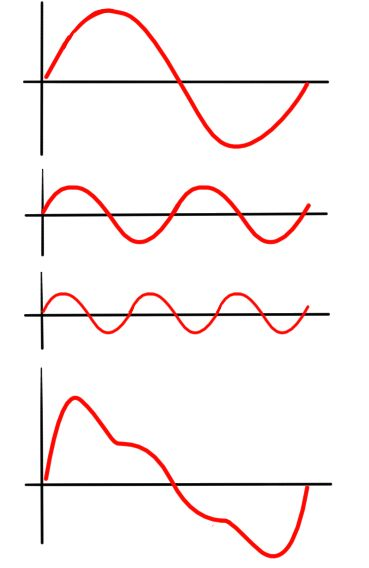
\includegraphics[height=2.5in]{images4/dispersion1.jpg}
\end{center}


  \end{frame}


%%%%%%%%%%%%%%%%%%%%%%%%%%%%%%%%%%%%%%%%%%%%%%%%%%%%%%%%%%%%%%%


\begin{frame}
\frametitle{Superposition Principle}

Example: the velocity of the waves depends on the frequency,

  \begin{center}
  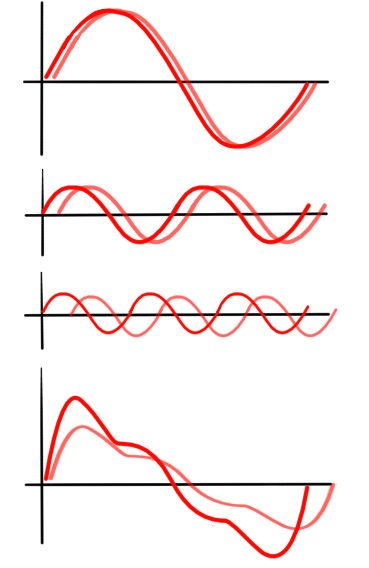
\includegraphics[height=2.5in]{images4/dispersion2.jpg}
\end{center}


  \end{frame}
%%%%%%%%%%%%%%%%%%%%%%%%%%%%%%%%%%%%%%%%%%%%%%%%%%%%%%%%%%%%%%%

\subsection{Reflection and transmission}
\begin{frame}
\frametitle{Reflection and transmission }

What happens when  a wave strikes an obstacle, or comes to the end of the medium in which it is
traveling?
\pause
\vspace{3mm}

At least a part of the wave is reflected.


  \end{frame}



%%%%%%%%%%%%%%%%%%%%%%%%%%%%%%%%%%%%%%%%%%%%%%%%%%%%%%%%%%%%%%%


\begin{frame}
\frametitle{Reflection and transmission }

Example:






   \begin{columns}[c]
   \column{2in}  % slides are 3in high by 5in wide


A wave pulse traveling down a cord is reflected as shown in the figure. The
reflected pulse returns inverted if the end of the cord is fixed; it
returns right side up if the end is free.

  
   \column{2in}

  \begin{center}
  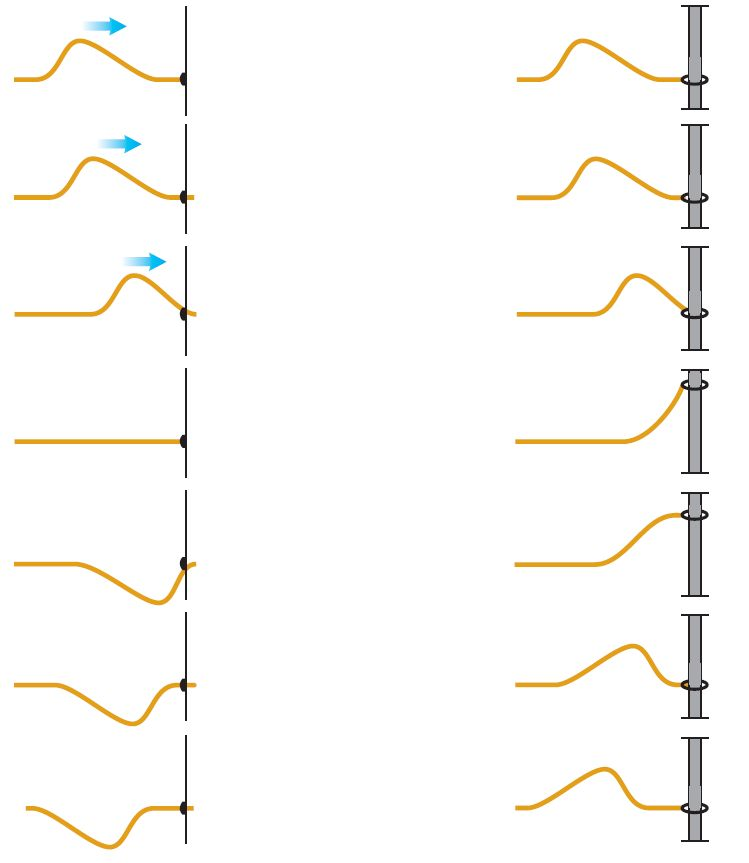
\includegraphics[height=2.3in]{images4/12.jpg}
\end{center}

   \end{columns}



  \end{frame}


%%%%%%%%%%%%%%%%%%%%%%%%%%%%%%%%%%%%%%%%%%%%%%%%%%%%%%%%%%%%%%%


\begin{frame}
\frametitle{Reflection and transmission }

  \begin{center}
  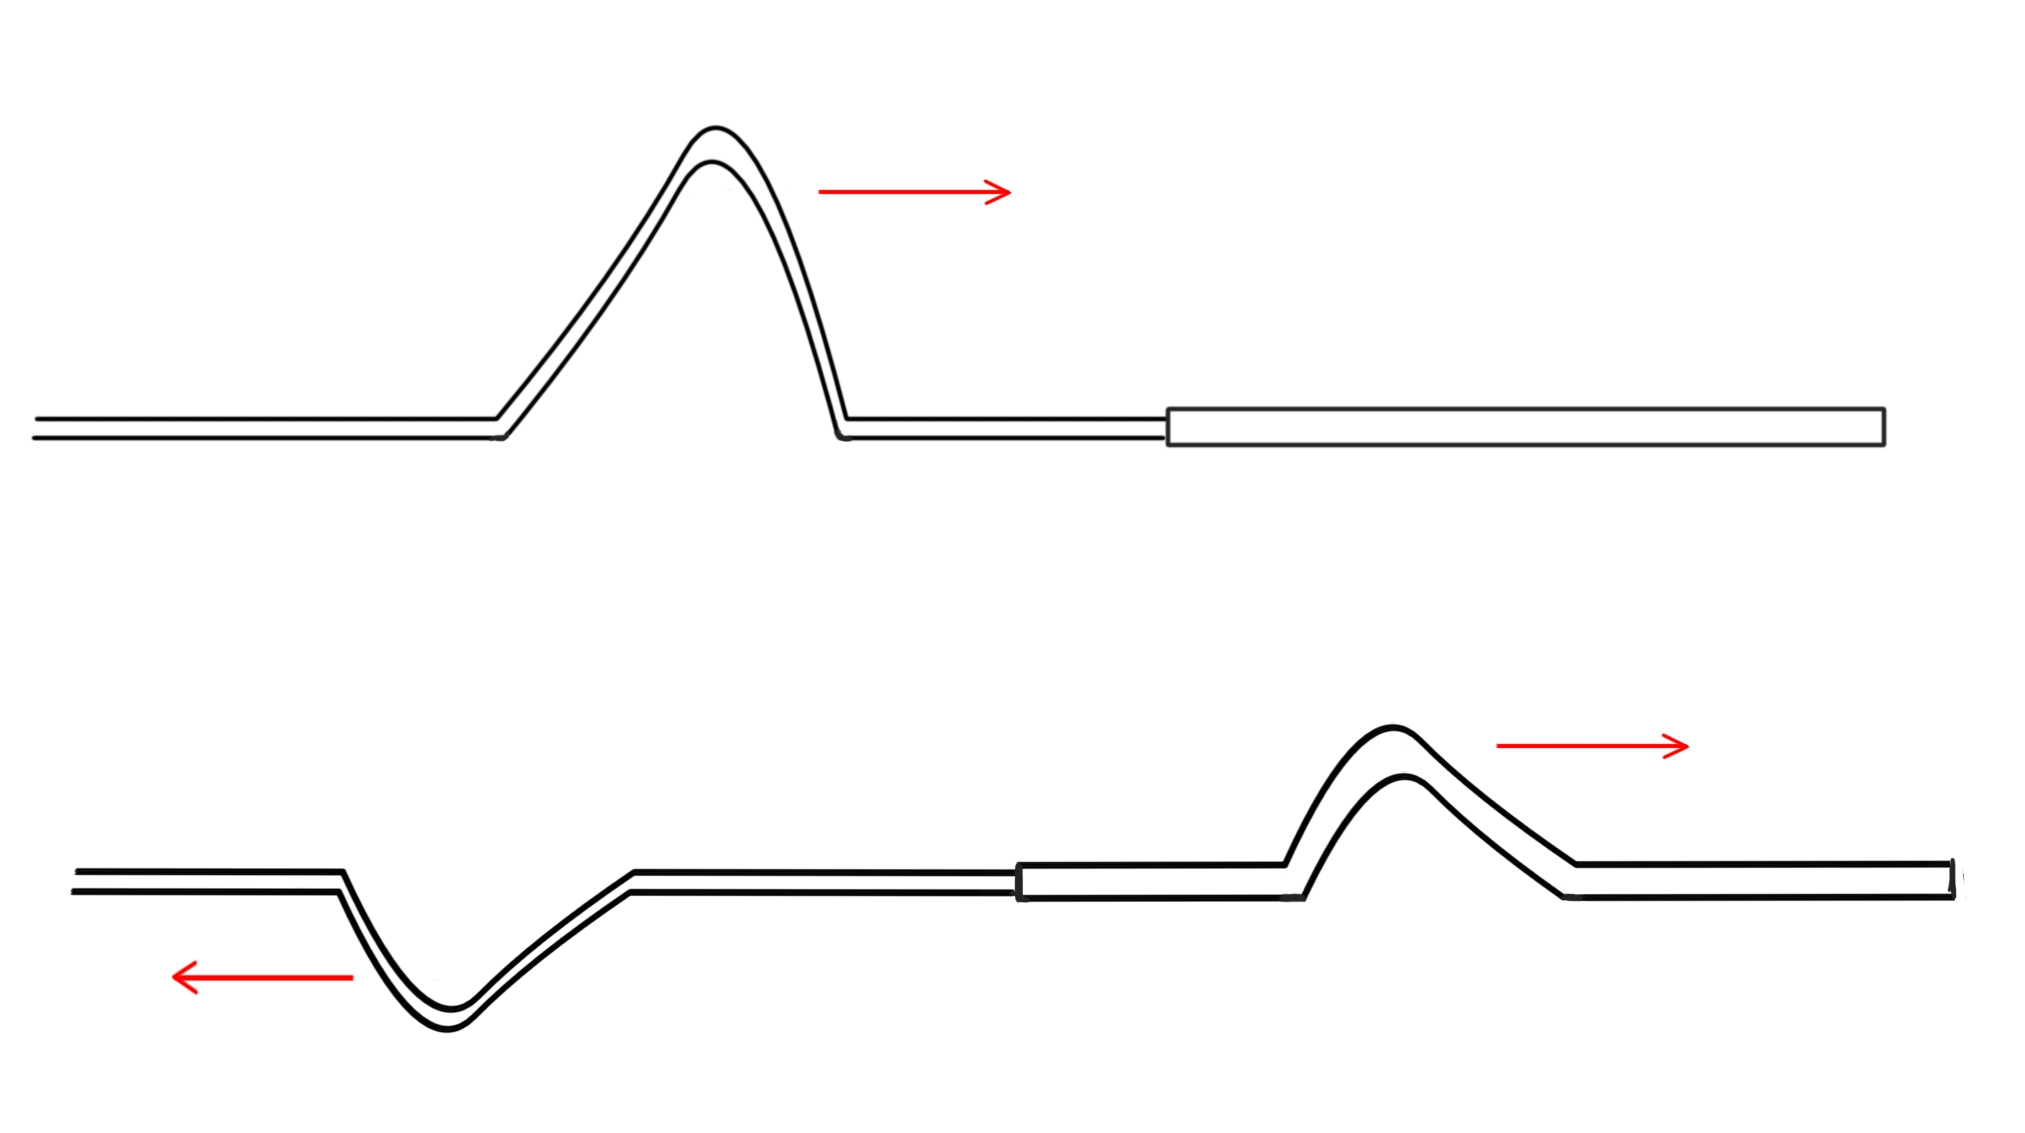
\includegraphics[height=2.5in]{images4/reflection.jpg}
\end{center}



  \end{frame}



%%%%%%%%%%%%%%%%%%%%%%%%%%%%%%%%%%%%%%%%%%%%%%%%%%%%%%%%%%%%%%%


\begin{frame}
\frametitle{Reflection and transmission }

Consider next a pulse that travels down a cord which consists of a light section
and a heavy section.  When the wave pulse reaches the
boundary between the two sections, part of the pulse is reflected and part is
transmitted. The heavier the second section of the cord, the less the
energy that is transmitted.


  \end{frame}





%%%%%%%%%%%%%%%%%%%%%%%%%%%%%%%%%%%%%%%%%%%%%%%%%%%%%%%%%%%%%%%


\begin{frame}
\frametitle{Reflection and transmission }




For a two- or three-dimensional wave, such as a water wave, we are concerned
with wave fronts, by which we mean all the points along the wave forming the
wave crest.



  \begin{center}
  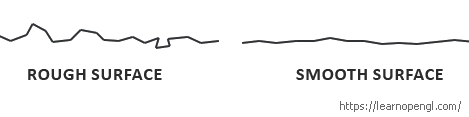
\includegraphics[height=1.7in]{images4/13.jpg}
\end{center}

  \end{frame}



%%%%%%%%%%%%%%%%%%%%%%%%%%%%%%%%%%%%%%%%%%%%%%%%%%%%%%%%%%%%%%%


\begin{frame}
\frametitle{Reflection and transmission }






A line drawn in the direction of motion, perpendicular to the wave front, is called a ray.



  \begin{center}
  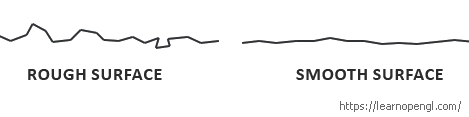
\includegraphics[height=1.7in]{images4/13.jpg}
\end{center}

  \end{frame}



%%%%%%%%%%%%%%%%%%%%%%%%%%%%%%%%%%%%%%%%%%%%%%%%%%%%%%%%%%%%%%%


\begin{frame}
\frametitle{Reflection and transmission }




Wave fronts far from the source have lost almost all their
curvature  and are nearly straight; they are
then called plane waves.


  \begin{center}
  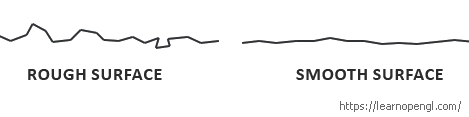
\includegraphics[height=1.7in]{images4/13.jpg}
\end{center}

  \end{frame}




%%%%%%%%%%%%%%%%%%%%%%%%%%%%%%%%%%%%%%%%%%%%%%%%%%%%%%%%%%%%%%%


\begin{frame}
\frametitle{Reflection and transmission }




For reflection of a two- or three-dimensional plane wave,
the angle that the incoming or incident wave makes with the reflecting surface is
equal to the angle made by the reflected wave. This is the\textbf{ law of reflection}:

\vspace{3mm}

\textbf{the angle of reflection equals the angle of incidence.}


  \begin{center}
  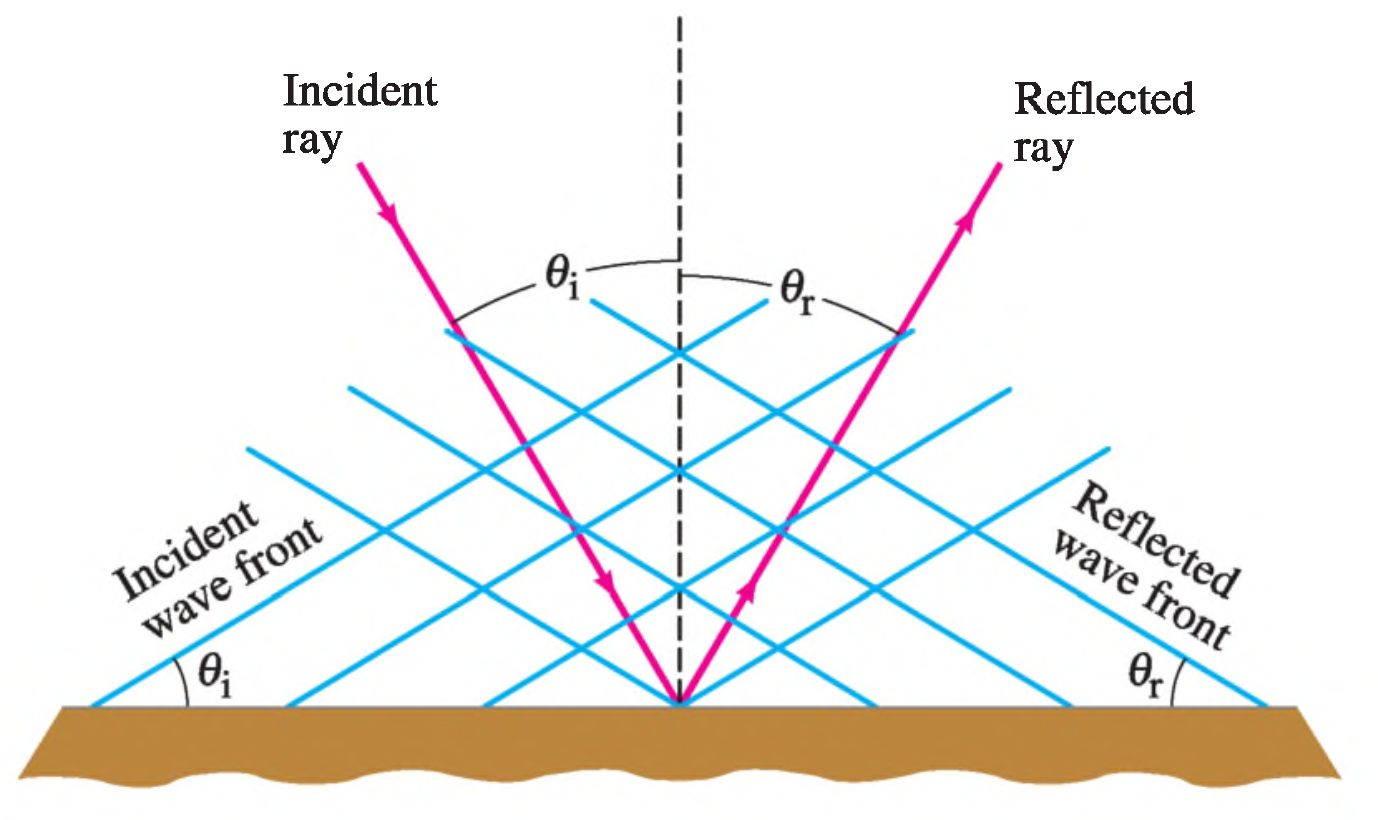
\includegraphics[height=1.5in]{images4/14.jpg}
\end{center}

  \end{frame}







%%%%%%%%%%%%%%%%%%%%%%%%%%%%%%%%%%%%%%%%%%%%%%%%%%%%%%%%%%%%%%%

\subsection{Interference}
\begin{frame}
\frametitle{Interference }




Interference refers to what happens when two waves pass through the same region
of space at the same time. In the region where they overlap, the resultant displacement is the algebraic sum of
their separate displacements.
\pause

\vspace{3mm}
We can have:

\pause
\begin{itemize}
\item \textbf{Destructive Interference} the two waves have opposite displacements at the instant they pass one another, and they
add to zero. 

\pause
\item \textbf{Constructive Interference} they produce a resultant displacement that is greater than the
displacement of either separate pulse,
\end{itemize}


  \end{frame}






%%%%%%%%%%%%%%%%%%%%%%%%%%%%%%%%%%%%%%%%%%%%%%%%%%%%%%%%%%%%%%%

\begin{frame}
\frametitle{Interference }

Example two pulses in a cord:




  \begin{center}
  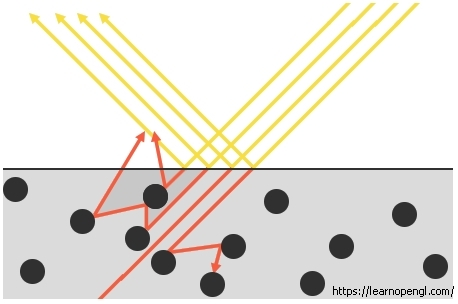
\includegraphics[height=1.8in]{images4/15.jpg}
\end{center}





  \end{frame}







%%%%%%%%%%%%%%%%%%%%%%%%%%%%%%%%%%%%%%%%%%%%%%%%%%%%%%%%%%%%%%%

\begin{frame}
\frametitle{Interference }

Example two rocks thrown simultaneously in water: 




  \begin{center}
  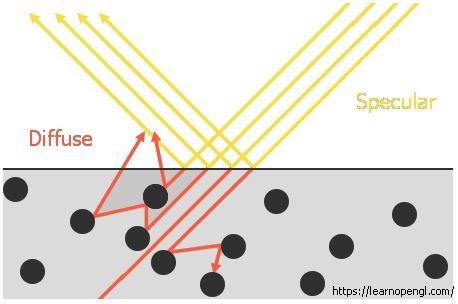
\includegraphics[height=2.3in]{images4/16.jpg}
\end{center}



  \end{frame}



%%%%%%%%%%%%%%%%%%%%%%%%%%%%%%%%%%%%%%%%%%%%%%%%%%%%%%%%%%%%%%%

\begin{frame}
\frametitle{Interference }

To summarize, the interference pattern of two equal waves can be constructive (waves is phase, phase $0$ degree), destructive (out of phase, phase $180$ degree), partially destructive
(other angles or different amplitudes).







  \begin{center}
  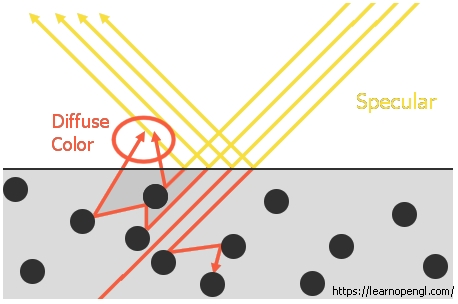
\includegraphics[height=1.4in]{images4/17.jpg}
\end{center}



  \end{frame}

%%%%%%%%%%%%%%%%%%%%%%%%%%%%%%%%%%%%%%%%%%%%%%%%%%%%%%%%%%%%%%%

\subsection{Standing waves  }
%%%%%%%%%%%%%%%%%%%%%%%%%%%%%%%%%%%%%%%%%%%%%%%%%%%%%%%%%%%%%%%






\begin{frame}
\frametitle{Resonance}

What happens when a string is pocked?


  \begin{center}
  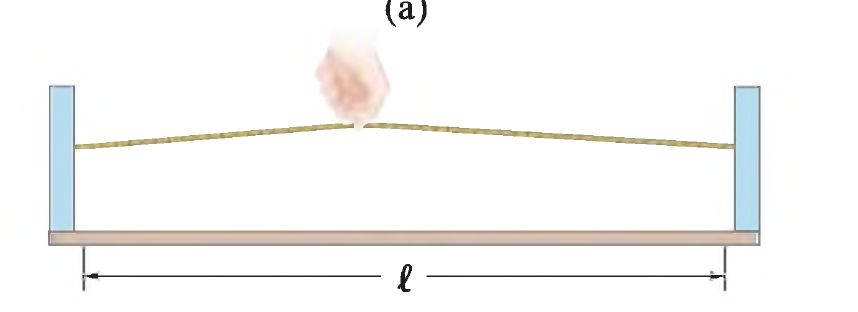
\includegraphics[height=1.4in]{images4/19.jpg}
\end{center}

\pause

The initial pulse is reflected in both extremes generating waves that travels in both direction that are reflected in the extremes and interfere.
  \end{frame}



\begin{frame}
\frametitle{Resonance}

A standing wave can be considered to consist of two traveling waves that
move in opposite directions.

\begin{equation*}
D(x,t)=D_1(x,t)+D_2(x,t)
\end{equation*}

\pause

\begin{equation*}
D_1(x,t)=Asin(kx-\omega t),~D_2(x,t)=Asin(kx+\omega t)
\end{equation*}


\begin{equation}
\rightarrow D(x,t)=2Asin(kx)cos(\omega t)
\end{equation}


  \end{frame}


%%%%%%%%%%%%%%%%%%%%%%%%%%%%%%%%%%%%%%%%%%%%%%%%%%%%%%%%%%%%%%%



\begin{frame}
\frametitle{Resonance}

If the string is fixed at its two ends,

\begin{equation*}
D(x=0,t)=D(x=\ell,t)=0
\end{equation*}
then,

\begin{equation}
 k\ell=n\pi \rightarrow k=\frac{ n\pi}{\ell}
\end{equation}

  \end{frame}





%%%%%%%%%%%%%%%%%%%%%%%%%%%%%%%%%%%%%%%%%%%%%%%%%%%%%%%%%%%%%%%



\begin{frame}
\frametitle{Resonance}


All particles of the string vibrate with
the same frequency,


\begin{equation*}
f=\frac{\omega}{2\pi}
\end{equation*}

but the amplitude depnds on $x$,


\begin{equation*}
amplitude=2Asin(kx)
\end{equation*}

The amplitude has a maximum, equal to $2A$, when

\begin{equation}
 kx=\frac{(2n+1)\pi}{2} \rightarrow x=\frac{(2 n+1)\pi}{k}
\end{equation}


  \end{frame}



\begin{frame}
\frametitle{Resonance}

The wavelengths of the
standing waves bear a simple relationship to the length $\ell$ of the string:

\begin{equation}
\lambda_n=\frac{2\ell}{n},~n=1~,2~,3,...
\end{equation}

\textbf{Fundamental frecuency}: $n=1\rightarrow \lambda_1$

\vspace{3mm}

\textbf{Harmonics}$\rightarrow  \lambda_n$

  \end{frame}



%%%%%%%%%%%%%%%%%%%%%%%%%%%%%%%%%%%%%%%%%%%%%%%%%%%%%%%%%%%%%%%

\begin{frame}
\frametitle{Resonance}

The frequency $f$ of each vibration is,


\begin{equation}
f_n=\frac{v}{\lambda_n}
\end{equation}

\pause

\begin{equation}
\rightarrow f_n=n \frac{v}{2\ell}
\end{equation}

\pause

And the velocity is,


\begin{equation*}
v=\sqrt{\frac{F_T}{\mu}}
\end{equation*}

  \end{frame}


%%%%%%%%%%%%%%%%%%%%%%%%%%%%%%%%%%%%%%%%%%%%%%%%%%%%%%%%%%%%%%%

\begin{frame}
\frametitle{Resonance}




The frequencies at which standing waves are produced are the \textbf{natural frequencies}
or \textbf{resonant frequencies} of the cord.



When a  string is plucked, only standing waves corresponding to resonant frequencies persist for long.



  \end{frame}







%%%%%%%%%%%%%%%%%%%%%%%%%%%%%%%%%%%%%%%%%%%%%%%%%%%%%%%%%%%%%%%







\begin{frame}
\frametitle{Resonance}



   \begin{columns}[c]
   \column{2.3in}  % slides are 3in high by 5in wide



Example: if you vibrate a
cord at just the right frequency, the cord simply appears to have
segments that oscillate up and down in a fixed pattern. The points of destructive
interference are called \textbf{nodes}. Points of
constructive interference  are called
\textbf{antinodes}. The nodes and antinodes remain in fixed positions for a particular frequency.
  
   \column{2.4in}



  \begin{center}
  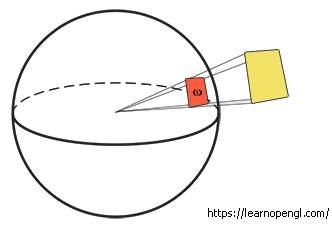
\includegraphics[height=2.4in]{images4/18.jpg}
\end{center}



   \end{columns}





  \end{frame}








%%%%%%%%%%%%%%%%%%%%%%%%%%%%%%%%%%%%%%%%%%%%%%%%%%%%%%%%%%%%%%%


\begin{frame}
\frametitle{Resonance}



  \begin{center}
  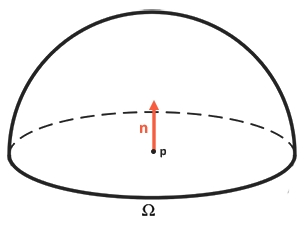
\includegraphics[height=2.4in]{images4/20.jpg}
\end{center}


  \end{frame}




%%%%%%%%%%%%%%%%%%%%%%%%%%%%%%%%%%%%%%%%%%%%%%%%%%%%%%%%%%%%%%%

\begin{frame}
\frametitle{Resonance}

 The term “standing” wave is also meaningful from the point of view
of energy. Since the string is at rest at the nodes, no energy flows past these points.
Hence the energy is not transmitted down the string but “stands” in place in the string.
\pause
\vspace{3mm}

Standing waves are produced not only on strings, but on any object that is
struck, such as a drum membrane or an object made of metal or wood.



  \end{frame}





%%%%%%%%%%%%%%%%%%%%%%%%%%%%%%%%%%%%%%%%%%%%%%%%%%%%%%%%%%%%%%%

\begin{frame}
\frametitle{Questions}

\begin{enumerate}
\item Is the frequency of a simple periodic wave equal to the
frequency of its source? Why or why not?

\pause
\item Describe how you could estimate the speed of water waves
across the surface of a pond.
\pause
\item Will any function of $(x- v t)$ represent a
wave motion? Why or why not? If not, give an example.
\pause

\item Is energy always conserved when two waves interfere?
Explain.
\pause
\item When a standing wave exists on a string, the vibrations of
incident and reflected waves cancel at the nodes. Does this
mean that energy was destroyed? Explain.

\pause

\item Can the amplitude of the standing waves  be
greater than the amplitude of the vibrations that cause them
(up and down motion of the hand)?


\end{enumerate}

  \end{frame}



%%%%%%%%%%%%%%%%%%%%%%%%%%%%%%%%%%%%%%%%%%%%%%%%%%%%%%%%%%%%%%%
\section{Sound}

\begin{frame}
\frametitle{Sound}

Is an interpretation of our brain of a physical sensation that stimulate our ears, that is, a longitudinal wave.

\pause

\vspace{3mm}

We must consider...

\pause
\begin{itemize}
\item Source $\rightarrow$ vibrating object.

\pause
\item Needs mater to spread.

\pause
\item The energy is transferred as longitudinal waves.

\pause
\item Detection $\rightarrow$ ears, microphone, etc.
\end{itemize}


  \end{frame}


%%%%%%%%%%%%%%%%%%%%%%%%%%%%%%%%%%%%%%%%%%%%%%%%%%%%%%%%%%%%%%%
\subsection{Characteristics}

\begin{frame}
\frametitle{Sound Speed}

The velocity of the propagation of sound in a medium is,

\begin{equation}
v=\sqrt{\frac{B}{\rho}}
\end{equation}

where $B$ is the Bulk modulus, defined by

\begin{equation*}
\Delta P=-B\frac{\Delta V}{V}
\end{equation*}

It relates the fractional change of volume due to a change in pressure. The minus sign means that the volume decreases if the pressure increases. 


 



  \end{frame}



%%%%%%%%%%%%%%%%%%%%%%%%%%%%%%%%%%%%%%%%%%%%%%%%%%%%%%%%%%%%%%%

\begin{frame}
\frametitle{Sound Speed}


  \begin{center}
  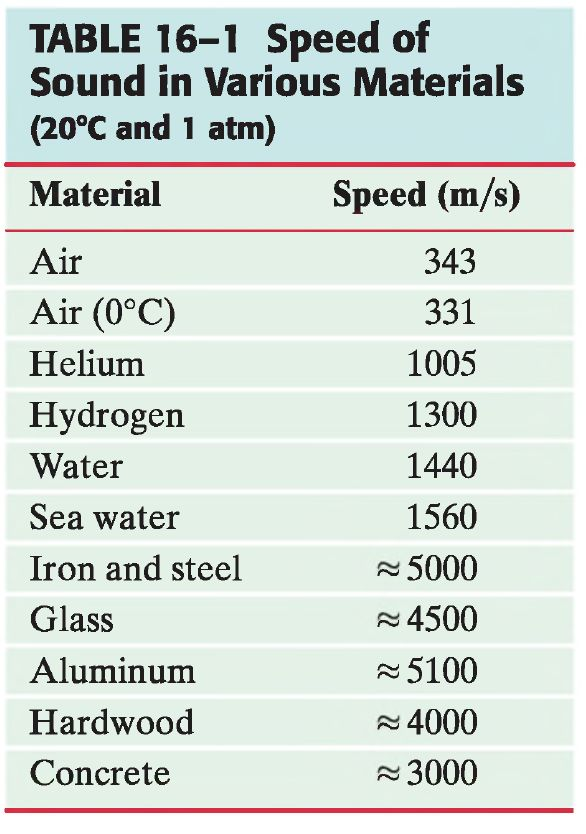
\includegraphics[height=2.4in]{images4/sound_speed.jpg}
\end{center}




  \end{frame}

%%%%%%%%%%%%%%%%%%%%%%%%%%%%%%%%%%%%%%%%%%%%%%%%%%%%%%%%%%%%%%%

\begin{frame}
\frametitle{Sound Characteristics}

To describe the sound, we have to consider two aspects,
\vspace{5mm}

\pause

\begin{itemize}
\item Loudness$\rightarrow$ Intensity ($\frac{E}{tS}$)
\pause

\item Pitch $\rightarrow$  high frequency/ low frequency
\end{itemize}

\pause

\vspace{3mm}

The audible range by humans  is $20$~Hz to $20000$~Hz

  \end{frame}

%%%%%%%%%%%%%%%%%%%%%%%%%%%%%%%%%%%%%%%%%%%%%%%%%%%%%%%%%%%%%%%
\subsection{Mathematical Description}


\begin{frame}
\frametitle{Pressure Waves}

A sound wave is a longitudinal wave described by,

\pause

\begin{equation*}
D=Asin(kx-\omega t)
\end{equation*}

\pause
  \begin{center}
  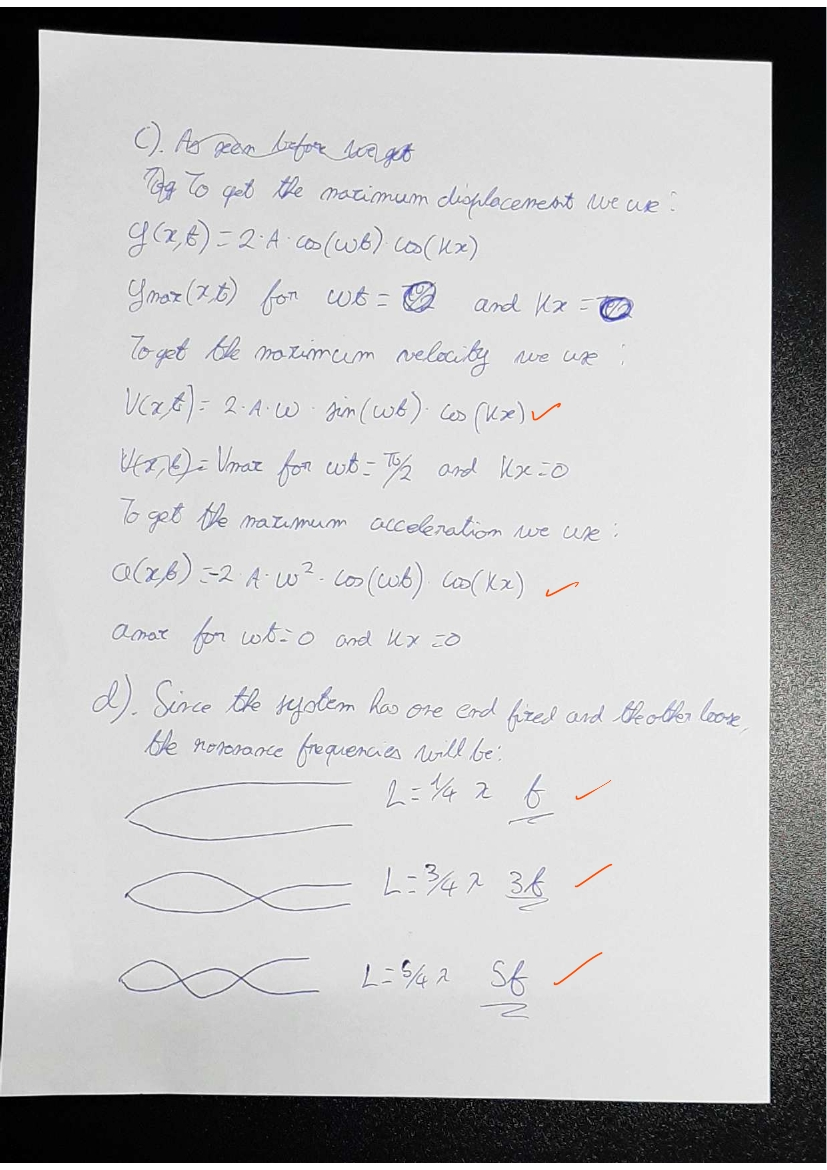
\includegraphics[height=2.in]{images4/5.jpg}
\end{center}

\pause
The variation of pressure is easier to measure.
  \end{frame}

%%%%%%%%%%%%%%%%%%%%%%%%%%%%%%%%%%%%%%%%%%%%%%%%%%%%%%%%%%%%%%%

\begin{frame}
\frametitle{Pressure Waves}

The displacement and pressure are $\frac{\pi}{2}$ out of phase.
  \begin{center}
  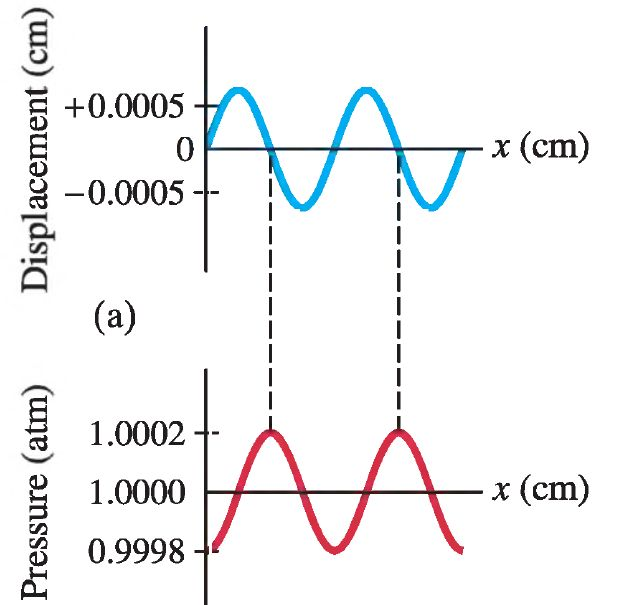
\includegraphics[height=2.in]{images4/soundwave.jpg}
\end{center}

  \end{frame}



%%%%%%%%%%%%%%%%%%%%%%%%%%%%%%%%%%%%%%%%%%%%%%%%%%%%%%%%%%%%%%%

\begin{frame}
\frametitle{Pressure Waves}
If we know the displacement function, $D(x,t)$, we can find the pressure wave using the definition of Bulk modulus,

\pause

\begin{equation*}
\Delta P=-B\frac{\Delta V}{V}
\end{equation*}

\pause

Let's consider a longitudinal wave crossing a certain volume element in a fluid,
\pause

   \begin{columns}[c]
   \column{1.8in}  % slides are 3in high by 5in wide
  
  \begin{center}
  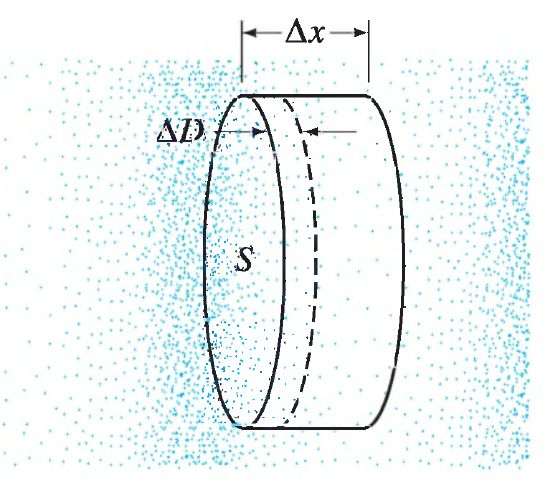
\includegraphics[height=1.3in]{images4/Pressurewave.jpg}
\end{center}

   \column{2.2in}
The volume is, $V=S\Delta x$.
\pause
\vspace{2mm}

The variation in volume due to the wave is: $\Delta V=S\Delta D$
\pause
\vspace{2mm}

The variation of pressure is..



\begin{equation}
\Delta P=-B\frac{S\Delta D}{S\Delta x}
\end{equation}


   \end{columns}




  \end{frame}
%%%%%%%%%%%%%%%%%%%%%%%%%%%%%%%%%%%%%%%%%%%%%%%%%%%%%%%%%%%%%%%

\begin{frame}
\frametitle{Pressure Waves}
Taking the limit for $\Delta x\rightarrow 0$

\begin{equation}
\Delta P=-B\frac{\partial  D}{\partial x}
\end{equation}

And...

\begin{equation}
\frac{\partial  D}{\partial x}=kA cos(kx-\omega t)
\end{equation}

Then,

\begin{equation}
\Delta P=-BkA cos(kx-\omega t)
\end{equation}

where the pressure amplitude is,


\begin{equation}
\Delta P_M=BkA 
\end{equation}

  \end{frame}



%%%%%%%%%%%%%%%%%%%%%%%%%%%%%%%%%%%%%%%%%%%%%%%%%%%%%%%%%%%%%%%

\begin{frame}
\frametitle{Pressure Waves}
Using the relations,


\begin{equation*}
v=\sqrt{\frac{B}{\rho}}, \ k=\frac{2\pi f}{v}
\end{equation*}

\begin{equation}
\Delta P_M=BkA =2\pi v \rho f A
\end{equation}

  \end{frame}
%%%%%%%%%%%%%%%%%%%%%%%%%%%%%%%%%%%%%%%%%%%%%%%%%%%%%%%%%%%%%%%

\begin{frame}
\frametitle{Intensity of sound}


We are going  to define a new measurement unit that relates the intensity with loudness.
\vspace{3mm}
\pause

\begin{equation*}
I=\frac{Energy}{time~Surface}, \ \ [I]=\frac{W}{m^2}
\end{equation*}


\begin{itemize}
\item Intensity $\rightarrow$ Physically meassurable quantity.
\pause

\item Loudness $\rightarrow$ Subjective sensation. 
\end{itemize}
\pause
\vspace{3mm}

In terms of intensity, the Human ear can hear  
\vspace{3mm}
\pause

form $10^{-12}~\frac{W}{m^2}$ to $1~\frac{W}{m^2}$.

\vspace{3mm}
\pause
Then, we are going to define this new unit  in log scale.

  \end{frame}







%%%%%%%%%%%%%%%%%%%%%%%%%%%%%%%%%%%%%%%%%%%%%%%%%%%%%%%%%%%%%%%

\begin{frame}
\frametitle{Decibel}

We are going to define one decibel ($1~dB$) as,
\pause

\begin{equation}
\beta~ (in dB)=10 log\frac{I}{I_0}
\end{equation}

\pause

where $log$ is in base $10$, and $I_0$ is the intensity of a chosen reference level.
\pause

\begin{equation}
I_0=10^{-12}~\frac{W}{m^2}, \ minimum~audible~intensity
\end{equation}

  \end{frame}



%%%%%%%%%%%%%%%%%%%%%%%%%%%%%%%%%%%%%%%%%%%%%%%%%%%%%%%%%%%%%%%

\begin{frame}
\frametitle{Decibel}

Example: 

\vspace{3mm}

What is  the level of a sound whose intensity is $I=10^{-10}$~$\frac{W}{m^2}$?

\pause

\begin{equation}
\beta =10 log\left(\frac{10^{-10}}{10^{-12}}\right)=10log100=20~dB
\end{equation}

\pause
\vspace{3mm}
At the threshold of hearing?  $I=10^{-12}$~$\frac{W}{m^2}$?

\begin{equation}
\beta =10 log\left(\frac{10^{-12}}{10^{-12}}\right)=10log1=0
\end{equation}

  \end{frame}

%%%%%%%%%%%%%%%%%%%%%%%%%%%%%%%%%%%%%%%%%%%%%%%%%%%%%%%%%%%%%%%

\begin{frame}
\frametitle{Decibel}

An increase in $I$ by a factor $10$ is equivalent to an increase in $10$~dB.
\pause

\begin{equation*}
I'=10I\rightarrow \beta'=10 log \frac{10I}{I_0}=10[log 10+log\frac{I}{I_0} ]
\end{equation*}
\pause
\begin{equation*}
\rightarrow\beta'=10~dB+10log\frac{I}{I_0} 
\end{equation*}
\pause

An increase in $I$ by a factor $10^2$ is equivalent to an increase in $20$~dB and so on...



  \end{frame}

%%%%%%%%%%%%%%%%%%%%%%%%%%%%%%%%%%%%%%%%%%%%%%%%%%%%%%%%%%%%%%%

\begin{frame}
\frametitle{Decibel}

  \begin{center}
  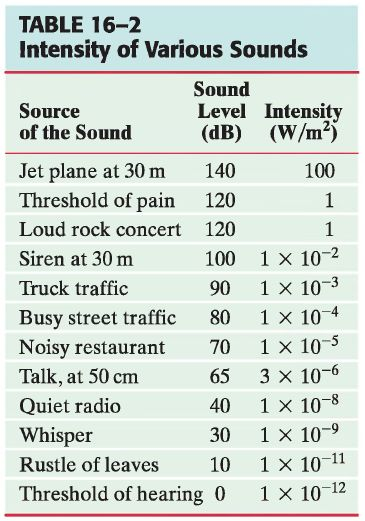
\includegraphics[height=2.5in]{images4/decibels.jpg}
\end{center}




  \end{frame}





%%%%%%%%%%%%%%%%%%%%%%%%%%%%%%%%%%%%%%%%%%%%%%%%%%%%%%%%%%%%%%%

\begin{frame}
\frametitle{Decibel}
Conceptual example:

\vspace{3mm}

A trumpeter plays at a sound level of $75~dB$. Three equally loud trumpet players join in. What is the new
sound level?

\pause

\begin{equation*}
\beta =10 log\frac{4 I_1}{I_0}
\end{equation*}


  \end{frame}




%%%%%%%%%%%%%%%%%%%%%%%%%%%%%%%%%%%%%%%%%%%%%%%%%%%%%%%%%%%%%%%

\begin{frame}
\frametitle{Decibel}
Conceptual example:

\vspace{3mm}

A trumpeter plays at a sound level of $75~dB$. Three equally loud trumpet players join in. What is the new
sound level?

\begin{equation*}
\beta =10 log\frac{4 I_1}{I_0}=10log(4)+10~log\frac{ I_1}{I_0}
\end{equation*}


  \end{frame}



%%%%%%%%%%%%%%%%%%%%%%%%%%%%%%%%%%%%%%%%%%%%%%%%%%%%%%%%%%%%%%%

\begin{frame}
\frametitle{Decibel}
Conceptual example:

\vspace{3mm}

A trumpeter plays at a sound level of $75~dB$. Three equally loud trumpet players join in. What is the new
sound level?

\begin{equation*}
\beta =10 log\frac{4 I_1}{I_0}=10log(4)+10~log\frac{ I_1}{I_0}=6.0~dB+75~dB=81~dB
\end{equation*}


  \end{frame}

%%%%%%%%%%%%%%%%%%%%%%%%%%%%%%%%%%%%%%%%%%%%%%%%%%%%%%%%%%%%%%%
\subsection{Sources of Sound}

\begin{frame}
\frametitle{Sources of Sound}

The source of any sound is a vibrating object.
\pause
\vspace{3mm}

In musical instruments, standing
waves are produced and the source vibrates at its natural resonant frequencies.
\pause
\vspace{3mm}

The vibrating source is in contact with the air (or other medium) and pushes on it to
produce sound waves that travel outward.
\vspace{3mm}
\pause

The frequencies of the waves are the same
as those of the source, but the speed and wavelengths can be different.



  \end{frame}



%%%%%%%%%%%%%%%%%%%%%%%%%%%%%%%%%%%%%%%%%%%%%%%%%%%%%%%%%%%%%%%



\begin{frame}
\frametitle{Equally Tempered Chromatic Scale}

The pitch of a pure sound is determined by the frequency. 


  \begin{center}
  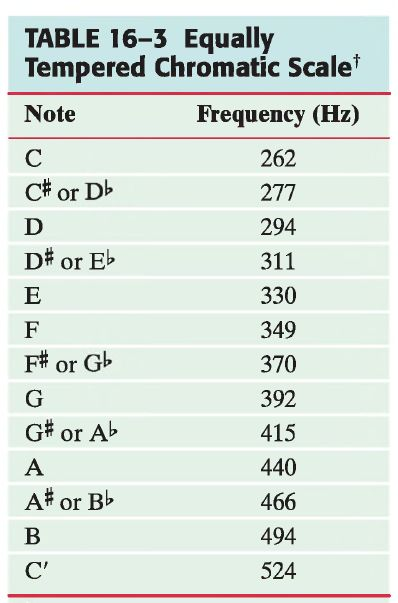
\includegraphics[height=2.3in]{images4/scale.jpg}
\end{center}



  \end{frame}



%%%%%%%%%%%%%%%%%%%%%%%%%%%%%%%%%%%%%%%%%%%%%%%%%%%%%%%%%%%%%%%



\begin{frame}
\frametitle{Stringed Instruments}

Standing waves are the basis for all stringed instruments.
\pause
\vspace{3mm}

The pitch is  determined by the lowest resonant frequency $\rightarrow$  nodes occurring only at the ends, $\lambda=2\ell$
\pause
\vspace{3mm}


Possible frequencies for standing waves:

\begin{equation}
f_n=nf_1=n\frac{v}{2\ell}
\end{equation}

\pause
\vspace{3mm}


When a finger is placed on the string of a guitar or violin, the effective length of
the string is shortened. So its fundamental frequency, and pitch, is higher since the
wavelength of the fundamental is shorter.




  \end{frame}

%%%%%%%%%%%%%%%%%%%%%%%%%%%%%%%%%%%%%%%%%%%%%%%%%%%%%%%%%%%%%%%



\begin{frame}
\frametitle{Stringed Instruments}


The strings on a guitar or violin are all the same length. Different $\mu\rightarrow$ different pitch

\pause


\begin{equation}
v=\sqrt{\frac{F_T}{\mu}}
\end{equation}

\vspace{3mm}
\pause

Thus the velocity on a heavier string is lower and the frequency will be lower for the
same wavelength.


\vspace{3mm}
\pause

The tension $F_T$ may also be different.  Adjusting the tension $\rightarrow$ tuning the pitch of each string.

\vspace{3mm}
\pause
  In pianos and harps the strings are of different lengths. For the lower notes the strings are not only longer, but heavier as well.

  \end{frame}






%%%%%%%%%%%%%%%%%%%%%%%%%%%%%%%%%%%%%%%%%%%%%%%%%%%%%%%%%%%%%%%



\begin{frame}
\frametitle{Piano Strings}

Example:

\vspace{3mm}

The highest key on a piano corresponds to a frequency about $150$ times that of the lowest key. If the string for the highest note
is $5.0~cm$ long, how long would the string for the lowest note have to be if it had the same mass per unit length and was under the same tension?

\pause

\begin{equation}
f_n=n\frac{v}{2\ell}
\end{equation}
\pause


\begin{equation}
\rightarrow \frac{\ell_L}{\ell_H}=\frac{f_H}{f_L}=150\rightarrow\ell_L=\frac{f_H}{f_L}=150\ell_H=750~cm
\end{equation}


  \end{frame}



%%%%%%%%%%%%%%%%%%%%%%%%%%%%%%%%%%%%%%%%%%%%%%%%%%%%%%%%%%%%%%%



\begin{frame}
\frametitle{Piano Strings}


The longer strings of lower frequency are made heavier, of higher mass
per unit length, so even on grand pianos the strings are less than 3 m long.

  \end{frame}


%%%%%%%%%%%%%%%%%%%%%%%%%%%%%%%%%%%%%%%%%%%%%%%%%%%%%%%%%%%%%%%



\begin{frame}
\frametitle{Example}

Frequencies and wavelengths in the violin:
\vspace{3mm}


A $0.32~m$ long violin string is tuned to play A above middle C at 440 Hz. (a) What is the
wavelength of the fundamental string vibration, and (b) what are the frequency
and wavelength of the sound wave produced? (c) Why is there a difference?

  \end{frame}


%%%%%%%%%%%%%%%%%%%%%%%%%%%%%%%%%%%%%%%%%%%%%%%%%%%%%%%%%%%%%%%



\begin{frame}
\frametitle{Sound Amplification}

Stringed instruments would not be very loud if they relied on their vibrating
strings to produce the sound waves since the strings are too thin to compress and
expand much air. Stringed instruments therefore make use of a kind of mechanical
amplifier known as a sounding board (piano) or sounding box (guitar, violin), which
acts to amplify the sound by putting a greater surface area in contact with the air.
\vspace{3mm}

When the strings are set into vibration, the sounding board or box is set
into vibration as well. Since it has much greater area in contact with the air, it can
produce a more intense sound wave. On an electric guitar, the sounding box is not
so important since the vibrations of the strings are amplified electronically.

  \end{frame}


%%%%%%%%%%%%%%%%%%%%%%%%%%%%%%%%%%%%%%%%%%%%%%%%%%%%%%%%%%%%%%%



\begin{frame}
\frametitle{Wind Instruments}

Instruments such as woodwinds, the brasses, and the pipe organ produce sound
from the vibrations of standing waves in a column of air within a tube.
\pause 
\vspace{3mm}

Standing waves can occur in the air of any cavity, but the frequencies present can be 
complicated.
\pause 
\vspace{3mm}

We are going to study a narrow tube of a flute or an organ pipe. 
\pause 
\vspace{3mm}

Source $\rightarrow$ vibrating reed / vibrating lip /  stream against one edge leading to turbulence
\pause 
\vspace{3mm}

The air within the tube vibrates with a variety of frequencies, but only frequencies that
correspond to standing waves will persist.

  \end{frame}


%%%%%%%%%%%%%%%%%%%%%%%%%%%%%%%%%%%%%%%%%%%%%%%%%%%%%%%%%%%%%%%



\begin{frame}
\frametitle{Wind Instruments}

 The air within the tube vibrates in the form of longitudinal standing waves. We can describe the waves either in terms of the flow of the displacement of air or in terms of the pressure.
\pause 
\vspace{3mm}

In terms of $D(x,t)$:
\vspace{3mm}

\begin{itemize}
\item The air at the closed end of a tube is a displacement node.
\vspace{3mm}
\pause

\item  The air near the open end of a tube there will be an antinode. 
\end{itemize}


 




  \end{frame}




%%%%%%%%%%%%%%%%%%%%%%%%%%%%%%%%%%%%%%%%%%%%%%%%%%%%%%%%%%%%%%%



\begin{frame}
\frametitle{Modes of vibration for an open tube}

The exact position of the antinode near the open end of a tube depends on the diameter of the tube.
\vspace{3mm}
\pause


Small diameter  compared to the length $\rightarrow$ the antinode occurs very close to
the end. 
\vspace{3mm}
\pause


The position of the antinode may also depend slightly on the wavelength and other factors.


  \end{frame}


%%%%%%%%%%%%%%%%%%%%%%%%%%%%%%%%%%%%%%%%%%%%%%%%%%%%%%%%%%%%%%%



\begin{frame}
\frametitle{Modes of vibration for an open tube}

  \begin{center}
  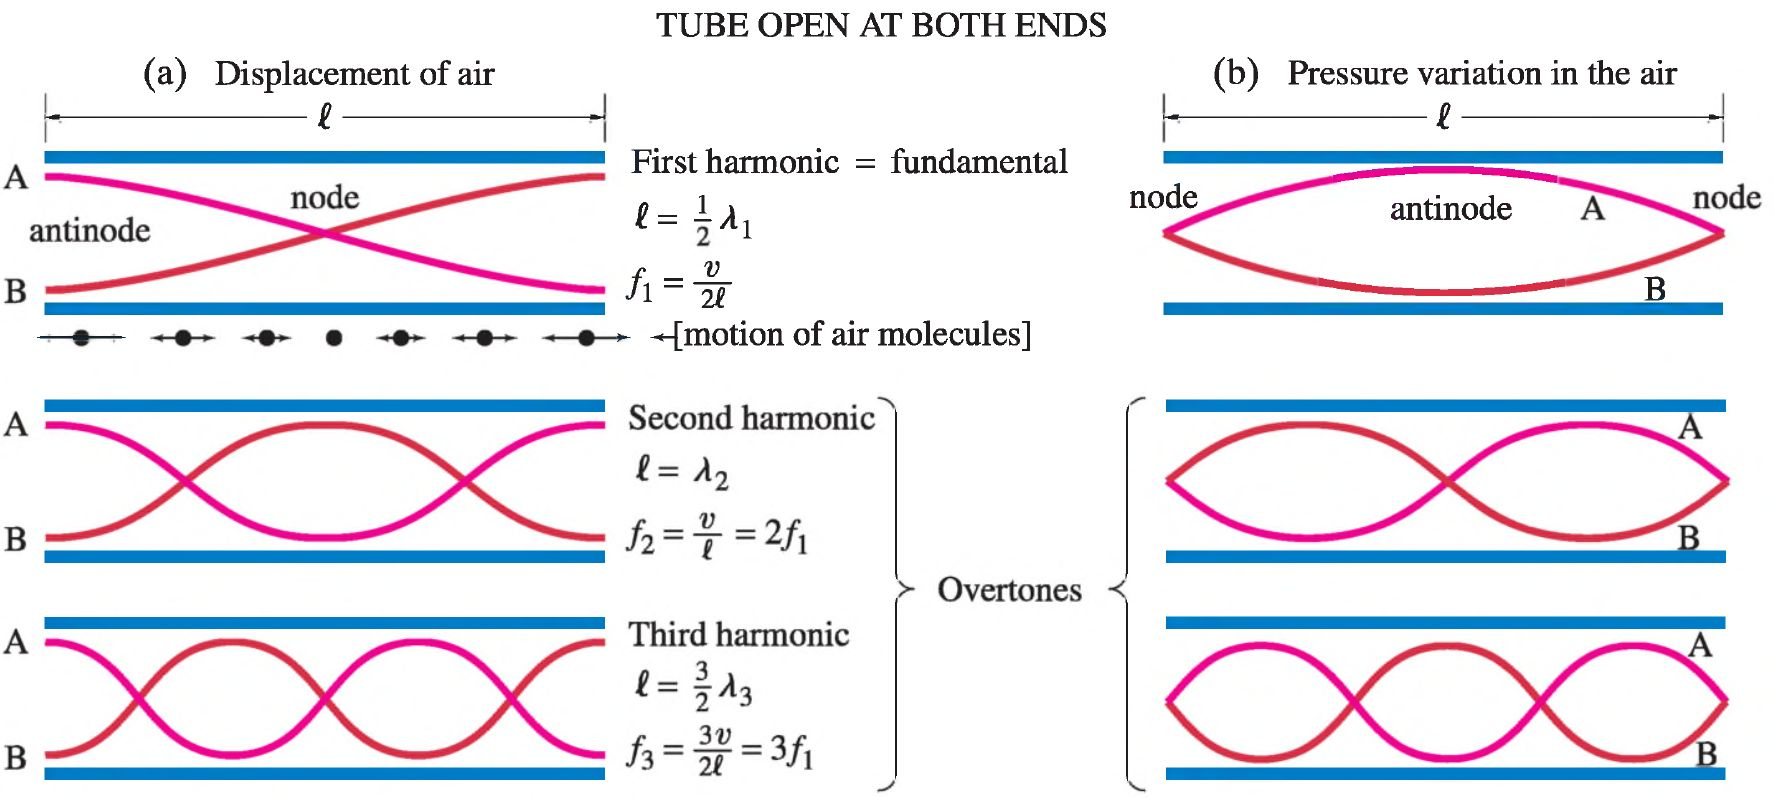
\includegraphics[height=2.in]{images4/tubeopen.jpg}
\end{center}


  \end{frame}




%%%%%%%%%%%%%%%%%%%%%%%%%%%%%%%%%%%%%%%%%%%%%%%%%%%%%%%%%%%%%%%



\begin{frame}
\frametitle{Modes of vibration for an open tube}

In terms of he displacement $D(x,t)$:

\begin{itemize}
\item Antinodes at both ends.
\pause
\item  There must be at least one node within an open tube.
if there is to be a standing wave at all.
\pause
\item Fundamental frequency $\rightarrow$ single node. 
\pause
\item Distance between two successive nodes (or antinodes),  is  $1/2\lambda\rightarrow \lambda=2\ell$.
\pause
\item Fundamental frequency: $f_0=v /\lambda=v/2\ell$, $v$ is the velocity of sound in the air.
\pause
\item  $f_n=n v /\lambda=n v/2\ell$.
\end{itemize}


  \end{frame}

%%%%%%%%%%%%%%%%%%%%%%%%%%%%%%%%%%%%%%%%%%%%%%%%%%%%%%%%%%%%%%%

\begin{frame}
\frametitle{Modes of vibration for a tube closed at one end}

  \begin{center}
  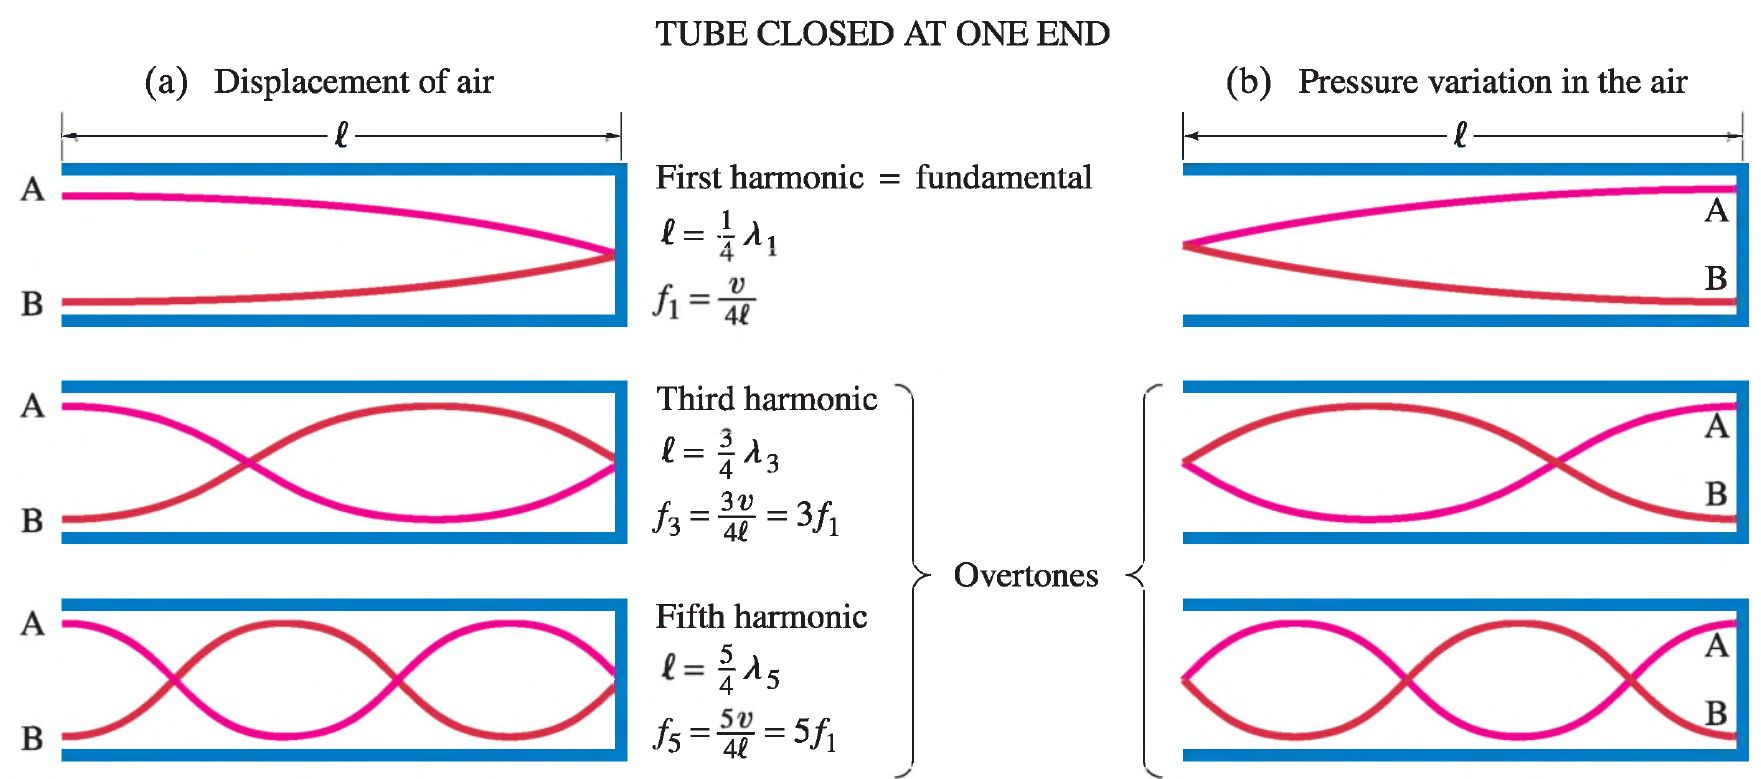
\includegraphics[height=2.in]{images4/tubeclose.jpg}
\end{center}


  \end{frame}


%%%%%%%%%%%%%%%%%%%%%%%%%%%%%%%%%%%%%%%%%%%%%%%%%%%%%%%%%%%%%%%

\begin{frame}
\frametitle{Modes of vibration for a tube closed at one end}

In terms of $D(x,t)$:
\vspace{3mm}

\begin{itemize}
\item There is always a displacement node at the closed end.
\pause
 
\item Distance between a node and the nearest antinode $\lambda/4$
\pause

\item Only the odd harmonics are present in a closed tube: the overtones have frequencies equal to $3f_1$,$5f_1$, $7f_1$,...
\pause

\item  There is no way for waves with $2f_1$, $4f_1$, $6f_1$


\end{itemize}



  \end{frame}




%%%%%%%%%%%%%%%%%%%%%%%%%%%%%%%%%%%%%%%%%%%%%%%%%%%%%%%%%%%%%%%



\begin{frame}
\frametitle{Modes of vibration for a tube closed at one end}

In terms of the pressure in the air:
\vspace{3mm}

\begin{itemize}

\item Air in a wave compressed $\rightarrow$ higher pressure.
\pause

\item Wave expansion (or rarefaction) $\rightarrow$ lower pressure.
\pause

\item The open end of a tube is open to the atmosphere $\rightarrow$ the pressure  remains at the outside atmospheric pressure (node).
\pause

\item  If a tube has a closed end  $\rightarrow$  the pressure  alternates to be above or below atmospheric pressure (antinode). 
\end{itemize}





  \end{frame}








%%%%%%%%%%%%%%%%%%%%%%%%%%%%%%%%%%%%%%%%%%%%%%%%%%%%%%%%%%%%%%%



\begin{frame}
\frametitle{Modes of vibration for a tube closed at one end}

Example:
\vspace{3mm}

Organ pipes. What will be the fundamental frequency and first
three overtones for a $26~cm$ long organ pipe at $20°C$  if it is (a) open and (b) closed?

  \end{frame}

%%%%%%%%%%%%%%%%%%%%%%%%%%%%%%%%%%%%%%%%%%%%%%%%%%%%%%%%%%%%%%%

\begin{frame}

\frametitle{Modes of vibration for a tube closed at one end}

Example:
\vspace{3mm}

A flute is designed to play middle C (262 Hz) as the
fundamental frequency when all the holes are covered. Approximately how long
should the distance be from the mouthpiece to the far end of the flute? (This is
only approximate since the antinode does not occur precisely at the mouthpiece.)
Assume the temperature is 20°C.

  \end{frame}
%%%%%%%%%%%%%%%%%%%%%%%%%%%%%%%%%%%%%%%%%%%%%%%%%%%%%%%%%%%%%%%

\begin{frame}
\frametitle{modes of vibration for an open tube}

Example:
\vspace{3mm}


To see why players of wind instruments “warm up” their instruments (so they
will be in tune), determine the fundamental frequency of the flute  when
all holes are covered and the temperature is 10°C instead of 20°C.


  \end{frame}


%%%%%%%%%%%%%%%%%%%%%%%%%%%%%%%%%%%%%%%%%%%%%%%%%%%%%%%%%%%%%%%


\subsection{Quality of Sound, and Noise;
Superposition}

\begin{frame}
\frametitle{Quality of sound}

We are aware of its loudness, its pitch, and also of a third aspect called its \textbf{timbre} or\textbf{ “quality”}.

\pause
\vspace{3mm}

For example, when a piano and then a flute play a note of the same loudness and pitch (say,
middle C), there is a clear difference in the overall sound. 

\pause
\vspace{3mm}

The quality of a sound depends on the presence of overtones, their
number and their relative amplitudes. Generally, when a note is played on a musical
instrument, the fundamental as well as overtones are present simultaneously.
\pause
\vspace{3mm}


Normally, more than two overtones are present. [Any complex wave can be analyzed
into a superposition of sinusoidal waves of appropriate amplitudes, wavelengths, and
frequencies ( Fourier)].


  \end{frame}






%%%%%%%%%%%%%%%%%%%%%%%%%%%%%%%%%%%%%%%%%%%%%%%%%%%%%%%%%%%%%%%


\begin{frame}
\frametitle{Sound spectra for different instruments}

  \begin{center}
  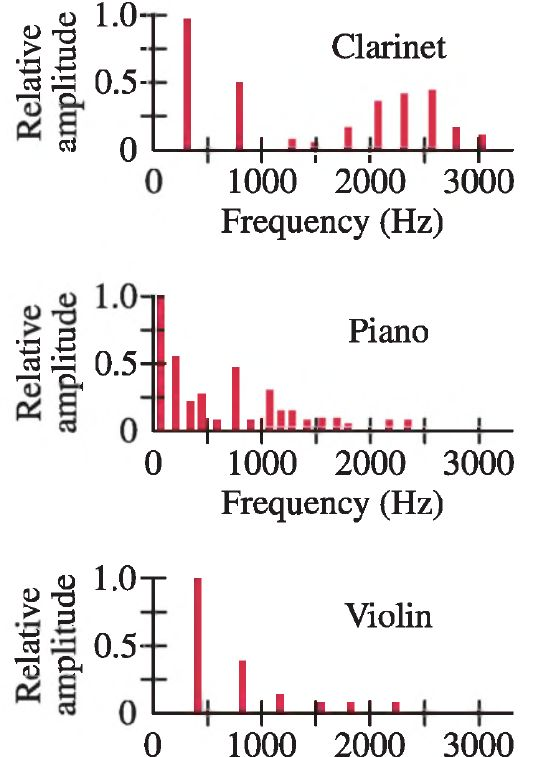
\includegraphics[height=2.5in]{images4/soundspectra.jpg}
\end{center}




  \end{frame}



%%%%%%%%%%%%%%%%%%%%%%%%%%%%%%%%%%%%%%%%%%%%%%%%%%%%%%%%%%%%%%%

\subsection{Interference of Sound Waves}
\begin{frame}
\frametitle{Spacial interference}

When two waves, with the same frequency, simultaneously pass through the
same region of space, they interfere with one another. Interference also occurs
with sound waves.



  \begin{columns}[c]
   \column{2in}  % slides are 3in high by 5in wide
  

  \begin{center}
  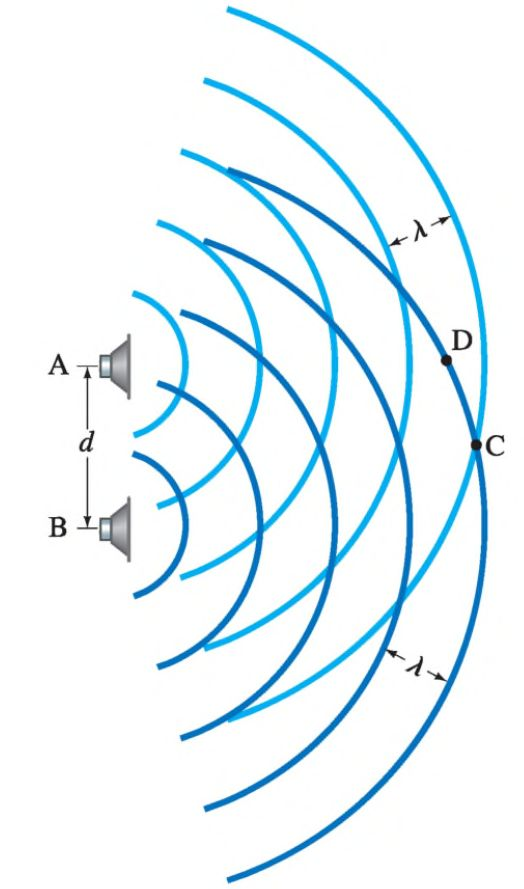
\includegraphics[height=1.8in]{images4/soundinterference.jpg}
\end{center}


   \column{2in}

\begin{itemize}
\item  Point C (same distance from each speaker) $rightarrow$ loud sound ( constructive interference).
\pause 

\item Point  D, no sound or  little sound  (destructive interference).
\end{itemize}


   \end{columns}
  \end{frame}








%%%%%%%%%%%%%%%%%%%%%%%%%%%%%%%%%%%%%%%%%%%%%%%%%%%%%%%%%%%%%%%

\begin{frame}
\frametitle{Spacial interference}


  \begin{columns}[c]
   \column{2in}  % slides are 3in high by 5in wide
  
  \begin{center}
  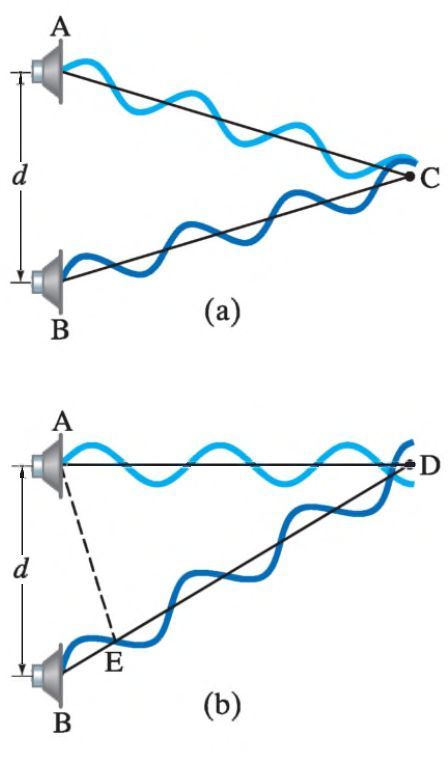
\includegraphics[height=2.in]{images4/soundinterference2.jpg}
\end{center}


   \column{2in}
\pause

  $ED=AD$,  If  $BE=\lambda/2$  the two waves will be exactly out of
phase when they reach D
\pause
\vspace{3mm}

 $\rightarrow$ destructive interference.

\pause
Then..

\begin{itemize}
\item $BD-AD=2\lambda, 3\lambda,...\rightarrow$ constructive interference
\pause

\item $BD-AD=\lambda/2, 3\lambda/2, 5\lambda/2,...\rightarrow$ destructive interference
\end{itemize}


   \end{columns}
  \end{frame}

%%%%%%%%%%%%%%%%%%%%%%%%%%%%%%%%%%%%%%%%%%%%%%%%%%%%%%%%%%%%%%%

\begin{frame}
\frametitle{Example}

Two loudspeakers are $1.00~m$
apart. A person stands $4.00~m$ from one speaker. How far must this person be
from the second speaker to detect destructive interference when the speakers
emit an 1150-Hz sound? Assume the temperature is 20°C.

  \end{frame}



%%%%%%%%%%%%%%%%%%%%%%%%%%%%%%%%%%%%%%%%%%%%%%%%%%%%%%%%%%%%%%%

\begin{frame}
\frametitle{Beats—Interference in Time}

 If two sources of sound are
close in frequency but not exactly the same, sound waves from the two sources interfere
with each other.
\pause
\vspace{3mm}

The sound level at a given position alternately rises and falls in time.
\pause
\vspace{3mm}


 The regularly spaced intensity changes are called beats.



  \end{frame}



%%%%%%%%%%%%%%%%%%%%%%%%%%%%%%%%%%%%%%%%%%%%%%%%%%%%%%%%%%%%%%%

\begin{frame}
\frametitle{Beats, Interference in Time}

  \begin{center}
  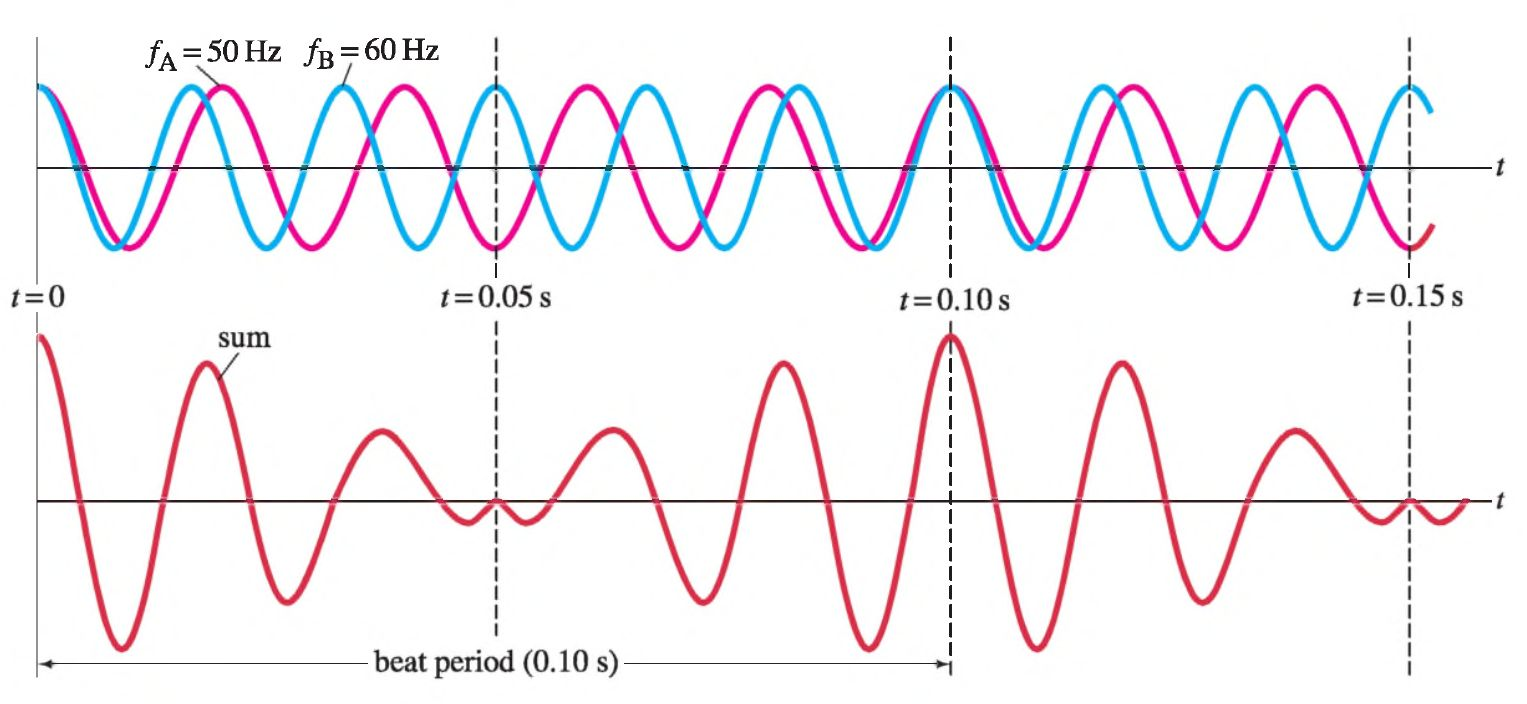
\includegraphics[height=1.7in]{images4/beats.jpg}
\end{center}


  \end{frame}



%%%%%%%%%%%%%%%%%%%%%%%%%%%%%%%%%%%%%%%%%%%%%%%%%%%%%%%%%%%%%%%

\begin{frame}
\frametitle{Beats, Interference in Time}


At a fixed point in space:

\begin{equation*}
D_1=Asin(2\pi f_1t)
\end{equation*}

\pause
\begin{equation*}
D_2=Asin(2\pi f_1t)
\end{equation*}
\pause

The resultant displacement is,

\pause

\begin{equation*}
D=D_1+D_2=A[Asin(2\pi f_1t)+sin(2\pi f_1t)]
\end{equation*}
\pause


  \end{frame}


%%%%%%%%%%%%%%%%%%%%%%%%%%%%%%%%%%%%%%%%%%%%%%%%%%%%%%%%%%%%%%%

\begin{frame}
\frametitle{Beats, Interference in Time}




Using, $sin\theta_1+sin\theta_2=2sin\frac{1}{2}(\theta_1+\theta_2)cos\frac{1}{2}(\theta_1-\theta_2)$

\pause

\begin{equation}
D=\left[2Acos2\pi\left(\frac{f_1-f_2}{2}\right)t\right] sin2\pi\left(\frac{f_1+f_2}{2}\right)t
\end{equation}

  \end{frame}



%%%%%%%%%%%%%%%%%%%%%%%%%%%%%%%%%%%%%%%%%%%%%%%%%%%%%%%%%%%%%%%

\begin{frame}
\frametitle{Beats, Interference in Time}


 The superposition of the two waves results in a wave that vibrates at the average frequency of the two components, $(f_1+ f_ 2)/2$.

\pause
\vspace{3mm}

 This
vibration has an amplitude given by the expression in brackets, and this amplitude varies
in time, from zero to a maximum of $2A$ , with a
frequency of$ (f_1 - f 2)/2$. 

\pause
\vspace{3mm}

A beat occurs whenever $cos2\pi\left(\frac{f_1-f_2}{2}\right)t$ equals $+1$ or$ -1$. 
\vspace{3mm}

\pause
$ \rightarrow$ two beats occur per cycle.Then  the beat frequency is $f_1-f_2$.


  \end{frame}







%%%%%%%%%%%%%%%%%%%%%%%%%%%%%%%%%%%%%%%%%%%%%%%%%%%%%%%%%%%%%%%

\begin{frame}
\frametitle{Example}

A tuning fork produces a steady $400~Hz$ tone. When this
tuning fork is struck and held near a vibrating guitar string, twenty beats are counted
in five seconds. What are the possible frequencies produced by the guitar string?

  \end{frame}






%%%%%%%%%%%%%%%%%%%%%%%%%%%%%%%%%%%%%%%%%%%%%%%%%%%%%%%%%%%%%%%
\subsection{Doppler Effect}

\begin{frame}
\frametitle{Doppler Effect}

Change in Pitch when a source of sound is moving toward or moving away from the observer. 

\pause
\vspace{3mm}

Source at rest $\rightarrow$ the wave travels at the velocity of sound in the air.

\pause

  \begin{center}
  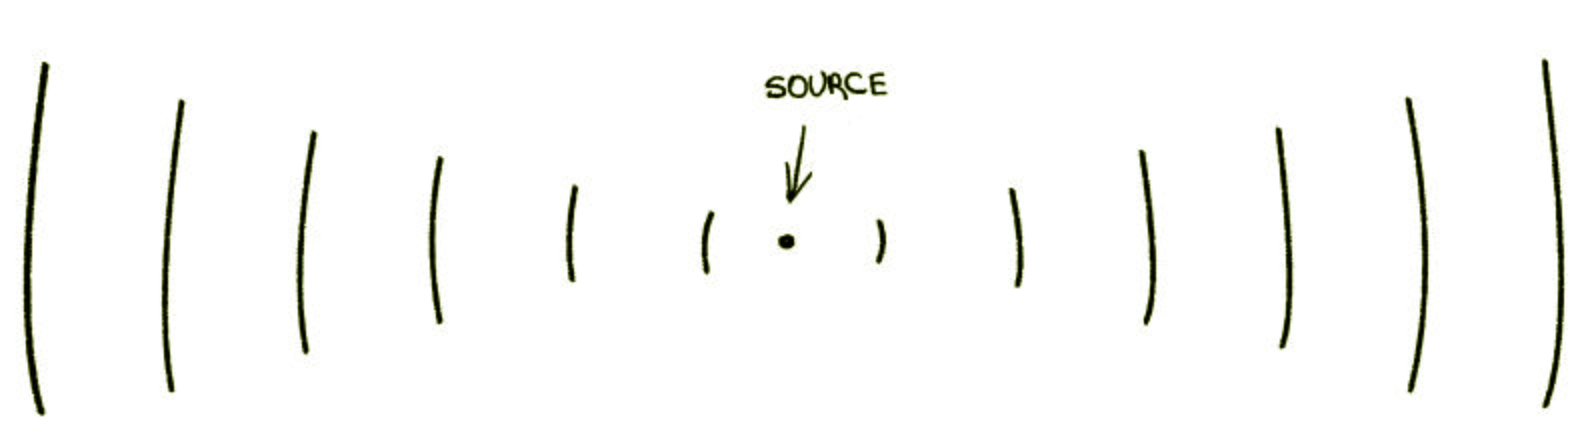
\includegraphics[height=1.2in]{images4/doppler1.jpg}
\end{center}


  \end{frame}





%%%%%%%%%%%%%%%%%%%%%%%%%%%%%%%%%%%%%%%%%%%%%%%%%%%%%%%%%%%%%%%

\begin{frame}
\frametitle{Doppler Effect}

Change in Pitch when a source of sound is moving toward or moving away from the observer. 

\vspace{3mm}

Source at rest $\rightarrow$ the wave travels at the velocity of sound in the air.



  \begin{center}
  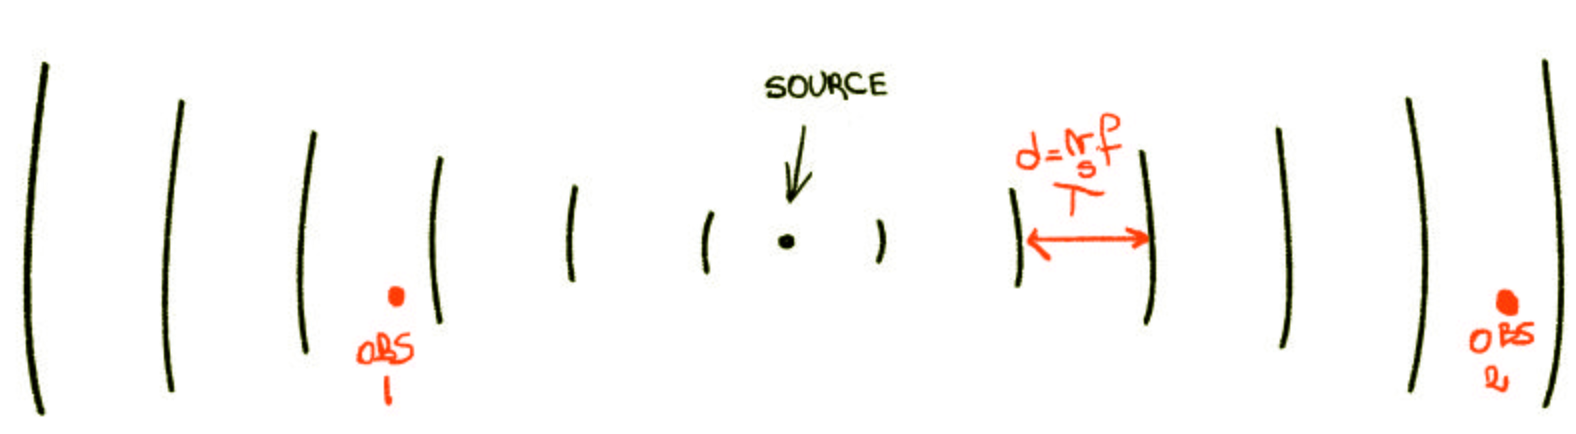
\includegraphics[height=1.2in]{images4/doppler2.jpg}
\end{center}


  \end{frame}






%%%%%%%%%%%%%%%%%%%%%%%%%%%%%%%%%%%%%%%%%%%%%%%%%%%%%%%%%%%%%%%
\begin{frame}
\frametitle{Doppler Effect}



Source in motion $\rightarrow$ the wave travels at the velocity of sound in the air (its velocity is independent of the source velocity).

\pause


  \begin{center}
  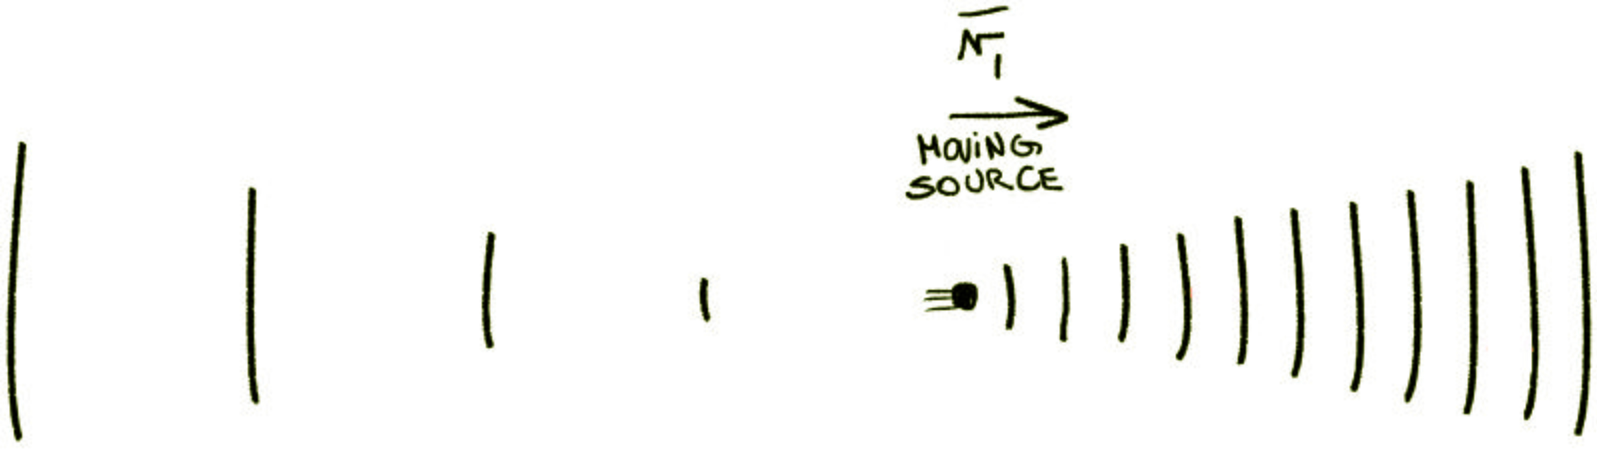
\includegraphics[height=1.2in]{images4/doppler3.jpg}
\end{center}


  \end{frame}

%%%%%%%%%%%%%%%%%%%%%%%%%%%%%%%%%%%%%%%%%%%%%%%%%%%%%%%%%%%%%%%


\begin{frame}
\frametitle{Doppler Effect}



Source in motion $\rightarrow$ the wave travels at the velocity of sound in the air (its velocity is independent of the source velocity).




  \begin{center}
  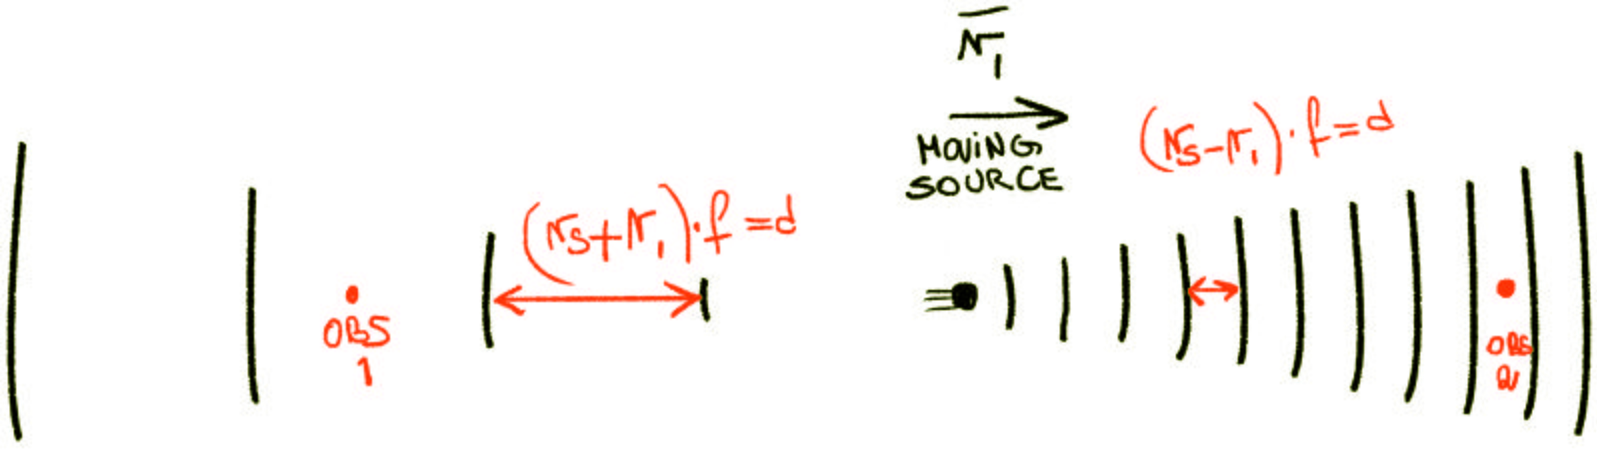
\includegraphics[height=1.2in]{images4/doppler4.jpg}
\end{center}


  \end{frame}



%%%%%%%%%%%%%%%%%%%%%%%%%%%%%%%%%%%%%%%%%%%%%%%%%%%%%%%%%%%%%%%

\begin{frame}
\frametitle{Doppler Effect}


The wavelength of a source traveling toward the observer is:

\begin{equation}
\lambda'=(v_{snd}-v_1)f
\end{equation}


  \end{frame}
%%%%%%%%%%%%%%%%%%%%%%%%%%%%%%%%%%%%%%%%%%%%%%%%%%%%%%%%%%%%%%%

\begin{frame}
\frametitle{Doppler Effect}


Then, the wavelength of a source traveling toward the observer is:

\begin{equation}
\lambda'=(v_{snd}-v_1)f=(v_{snd}-v_{source})\frac{\lambda}{v_{snd}}
\end{equation}


  \end{frame}
%%%%%%%%%%%%%%%%%%%%%%%%%%%%%%%%%%%%%%%%%%%%%%%%%%%%%%%%%%%%%%%

\begin{frame}
\frametitle{Doppler Effect}


Then, the wavelength of a source traveling toward the observer is:

\begin{equation}
\lambda'=(v_{snd}-v_{source})f=(v_{snd}-v_{source})\frac{\lambda}{v_{snd}}=\lambda(1-\frac{v_{source}}{v_{snd}})
\end{equation}

\pause

Where we consider that the source velocity is lower than the sound velocity. 
  \end{frame}

%%%%%%%%%%%%%%%%%%%%%%%%%%%%%%%%%%%%%%%%%%%%%%%%%%%%%%%%%%%%%%%

\begin{frame}
\frametitle{Doppler Effect}


Then, the shift in wavelength is,

\pause
\begin{equation}
\Delta \lambda=-\lambda \frac{v_{source}}{v_{snd}},
\end{equation}
\pause

proportional to the source velocity.

  \end{frame}
%%%%%%%%%%%%%%%%%%%%%%%%%%%%%%%%%%%%%%%%%%%%%%%%%%%%%%%%%%%%%%%

\begin{frame}
\frametitle{Doppler Effect}


The frequency perceived by the observer is,

\begin{equation}
f'=\frac{v_{snd}}{\lambda '}=\frac{v_{snd}}{\lambda(1-\frac{v_{source}}{v_{snd}})}
\end{equation}


  \end{frame}

%%%%%%%%%%%%%%%%%%%%%%%%%%%%%%%%%%%%%%%%%%%%%%%%%%%%%%%%%%%%%%%

\begin{frame}
\frametitle{Doppler Effect}


The frequency perceived by the observer is,

\begin{equation}
f'=\frac{f}{(1-\frac{v_{source}}{v_{snd}})}
\end{equation}


The denominator is less than 1, then the observed frequency is grater than the source frequency.

  \end{frame}






%%%%%%%%%%%%%%%%%%%%%%%%%%%%%%%%%%%%%%%%%%%%%%%%%%%%%%%%%%%%%%%

\begin{frame}
\frametitle{Doppler Effect}


If the source is moving away the observer,

\begin{equation}
\lambda'=(v_{snd}+v_{source})f=\lambda(1+\frac{v_{source}}{v_{snd}})
\end{equation}

\pause

The frequency is perceived by the observer is,

\pause

\begin{equation}
f'=\frac{f}{(1+\frac{v_{source}}{v_{snd}})}
\end{equation}

\pause

The observed frequency in this case is higher than the source frequency.


  \end{frame}





%%%%%%%%%%%%%%%%%%%%%%%%%%%%%%%%%%%%%%%%%%%%%%%%%%%%%%%%%%%%%%%

\begin{frame}
\frametitle{Doppler Effect}


What happens if the source is at rest and the observer is moving toward the source?

\pause

  \begin{center}
  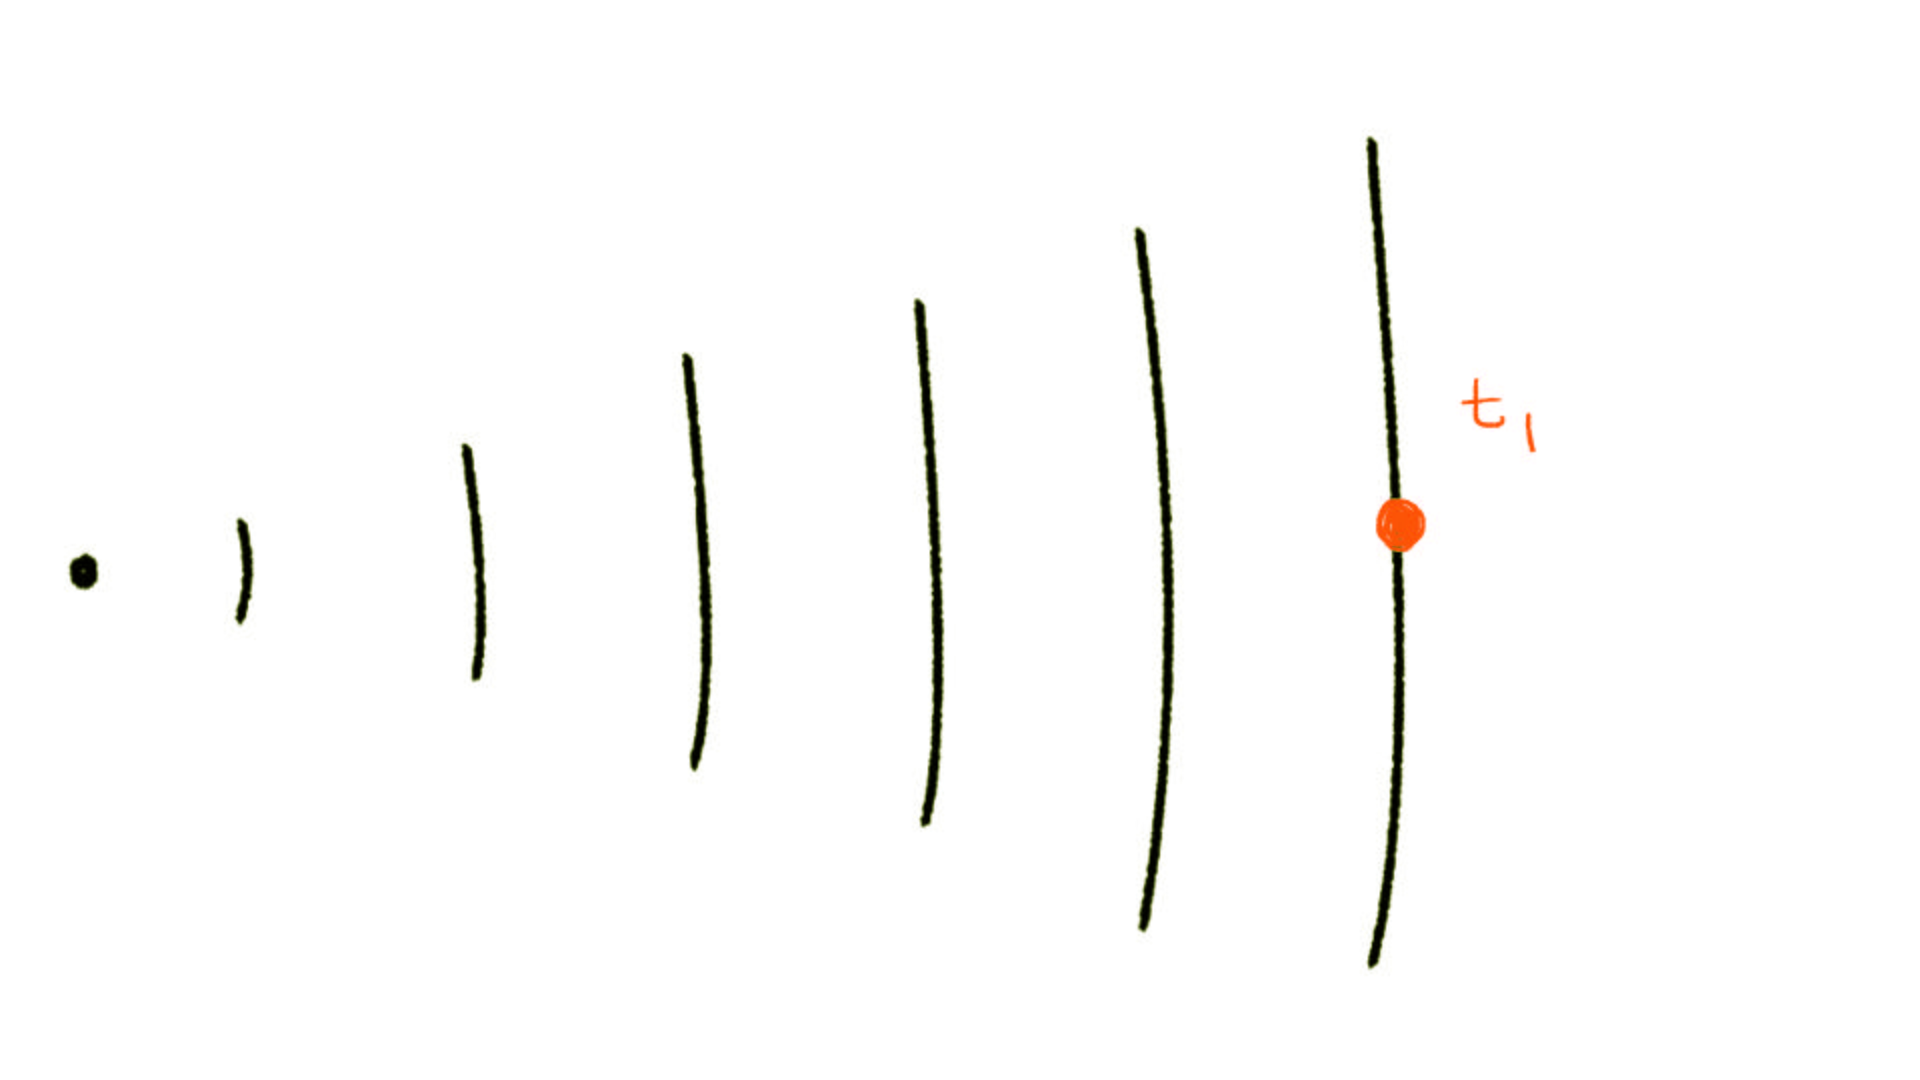
\includegraphics[height=1.2in]{images4/doppler5.jpg}
\end{center}


  \end{frame}



%%%%%%%%%%%%%%%%%%%%%%%%%%%%%%%%%%%%%%%%%%%%%%%%%%%%%%%%%%%%%%%

\begin{frame}
\frametitle{Doppler Effect}


What happens if the source is at rest and the observer is moving toward the source?



  \begin{center}
  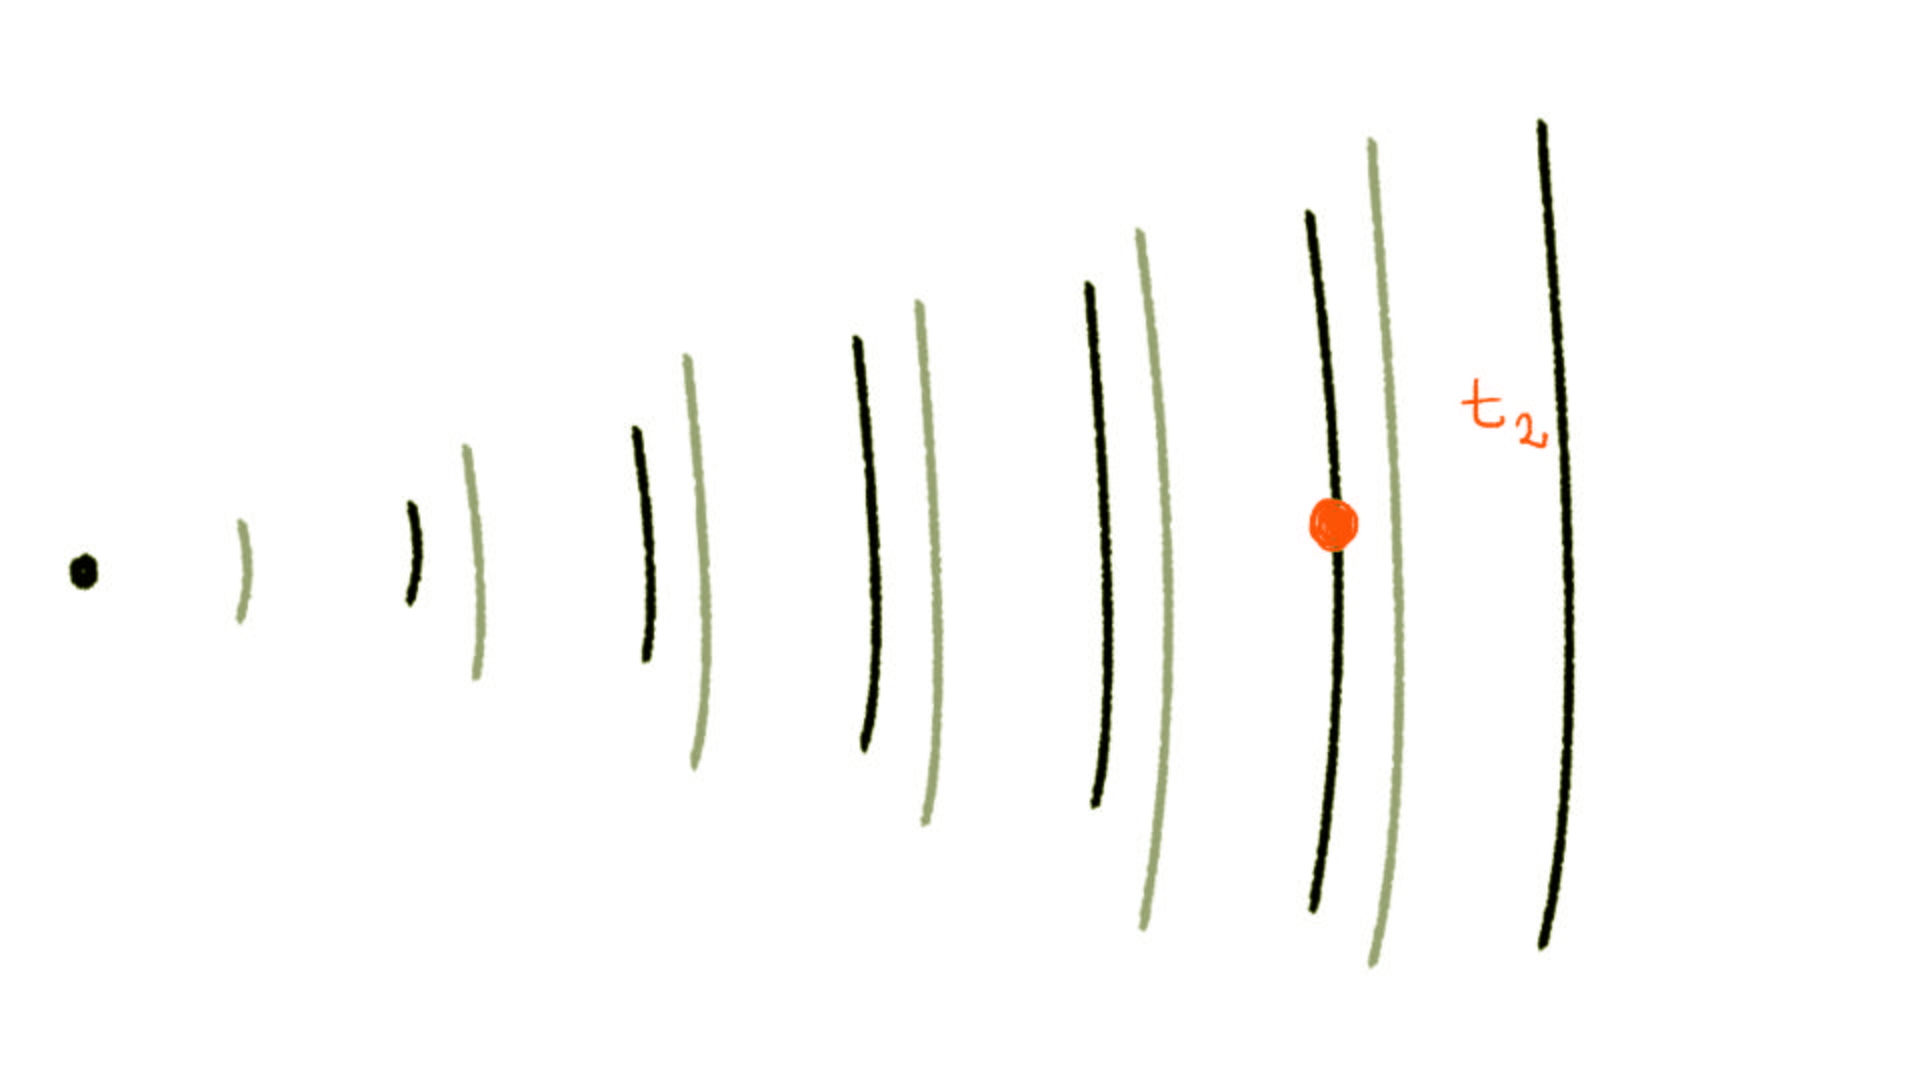
\includegraphics[height=1.2in]{images4/doppler6.jpg}
\end{center}


  \end{frame}







%%%%%%%%%%%%%%%%%%%%%%%%%%%%%%%%%%%%%%%%%%%%%%%%%%%%%%%%%%%%%%%

\begin{frame}
\frametitle{Doppler Effect}


What is the frequency perceived by the observer that is moving toward the source?

\begin{equation}
f'=\frac{v_{snd}+v_{obs}}{\lambda}
\end{equation}



  \end{frame}










%%%%%%%%%%%%%%%%%%%%%%%%%%%%%%%%%%%%%%%%%%%%%%%%%%%%%%%%%%%%%%%

\begin{frame}
\frametitle{Doppler Effect}


What is the frequency perceived by the observer that is moving toward the source?

\begin{equation}
f'=\frac{v_{snd}+v_{obs}}{\lambda}=f\left(1+\frac{v_{obs}}{v_{sound}}\right)
\end{equation}



\pause


Quantitatively the change in frequency is different
than for the case of a moving source. 



  \end{frame}




%%%%%%%%%%%%%%%%%%%%%%%%%%%%%%%%%%%%%%%%%%%%%%%%%%%%%%%%%%%%%%%

\begin{frame}
\frametitle{Doppler Effect}





Quantitatively the change in frequency is different
than for the case of a moving source. 

\pause
\vspace{3mm}

\begin{itemize}
\item Fixed source and a moving observer $\rightarrow$ $\lambda$ is not changed, but the velocity of the crest respect to the observer changes.
\item Moving source and fixed observer  $\rightarrow$ $\lambda$ changes, but the velocity of the crest respect to the observer does not change. 
\end{itemize}

  \end{frame}




%%%%%%%%%%%%%%%%%%%%%%%%%%%%%%%%%%%%%%%%%%%%%%%%%%%%%%%%%%%%%%%

\begin{frame}
\frametitle{Doppler Effect}



If the observer is moving away from the source, the velocity of the crests respect to the observer is decreased, and the frequency is,


\begin{equation}
f'=\frac{v_{snd}-v_{obs}}{\lambda}=f\left(1-\frac{v_{obs}}{v_{sound}}\right)
\end{equation}

  \end{frame}









%%%%%%%%%%%%%%%%%%%%%%%%%%%%%%%%%%%%%%%%%%%%%%%%%%%%%%%%%%%%%%%

\begin{frame}
\frametitle{Doppler Effect}


When a sound wave is reflected from a moving obstacle, the frequency of the
reflected wave will, because of the Doppler effect, be different from that of
the incident wave.



  \end{frame}


%%%%%%%%%%%%%%%%%%%%%%%%%%%%%%%%%%%%%%%%%%%%%%%%%%%%%%%%%%%%%%%

\begin{frame}
\frametitle{Doppler Effect}

Example: 

\vspace{3mm}

Two Doppler shifts. A $5000~Hz$ sound wave is emitted by a
stationary source. This sound wave reflects from an object moving $3.50~m/s$
toward the source. What is the frequency of the wave reflected by
the moving object as detected by a detector at rest near the source?




  \end{frame}



%%%%%%%%%%%%%%%%%%%%%%%%%%%%%%%%%%%%%%%%%%%%%%%%%%%%%%%%%%%%%%%

\begin{frame}
\frametitle{Doppler Effect}

Example: 

\vspace{3mm}

   \begin{columns}[c]
   \column{2in}  % slides are 3in high by 5in wide
  \begin{center}
  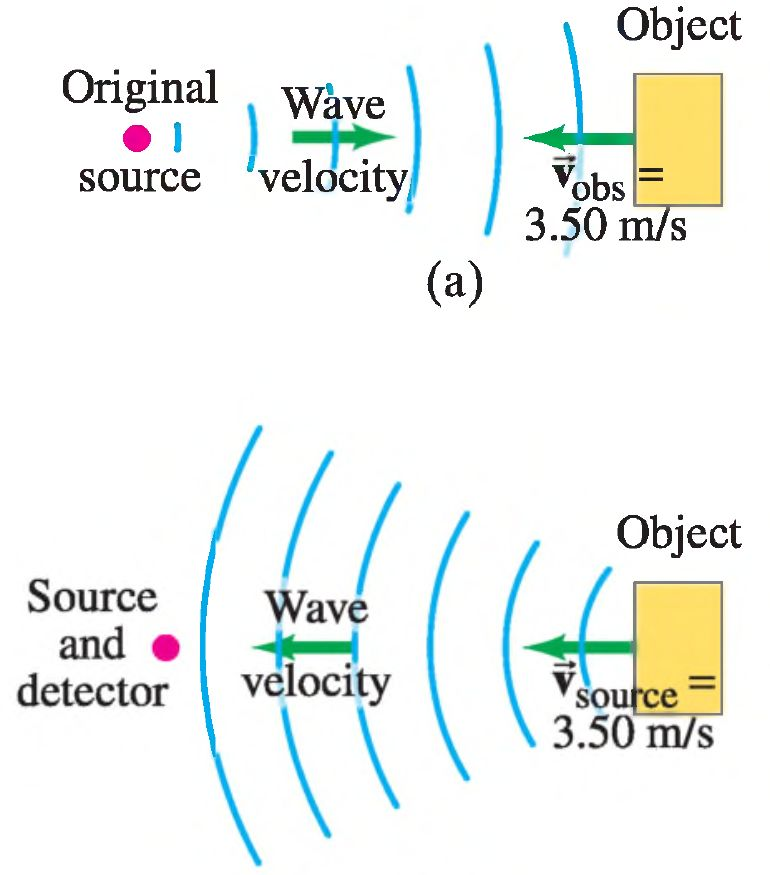
\includegraphics[height=2.in]{images4/doppler7.jpg}
\end{center}


  
   \column{2in}
\pause
The frequency detected by the observer is:

\begin{equation*}
f'= f\left(1+\frac{v_{obs}}{v_{sound}}\right)
\end{equation*}




   \end{columns}




  \end{frame}

%%%%%%%%%%%%%%%%%%%%%%%%%%%%%%%%%%%%%%%%%%%%%%%%%%%%%%%%%%%%%%%

\begin{frame}
\frametitle{Doppler Effect}

Example: 

\vspace{3mm}

   \begin{columns}[c]
   \column{2in}  % slides are 3in high by 5in wide
  \begin{center}
  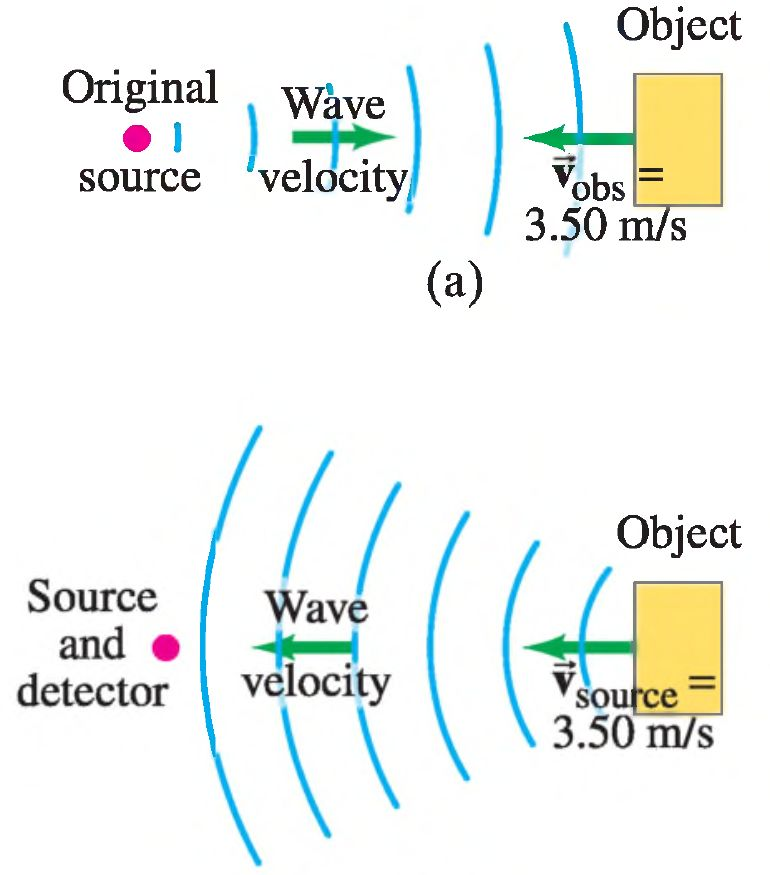
\includegraphics[height=2.in]{images4/doppler7.jpg}
\end{center}


  
   \column{2in}
\pause
The frequency detected by the observer is:

\begin{equation*}
f'= f\left(1+\frac{v_{obs}}{v_{sound}}\right)=5051~Hz
\end{equation*}




   \end{columns}




  \end{frame}


%%%%%%%%%%%%%%%%%%%%%%%%%%%%%%%%%%%%%%%%%%%%%%%%%%%%%%%%%%%%%%%

\begin{frame}
\frametitle{Doppler Effect}

Example: 

\vspace{3mm}

   \begin{columns}[c]
   \column{2in}  % slides are 3in high by 5in wide
  \begin{center}
  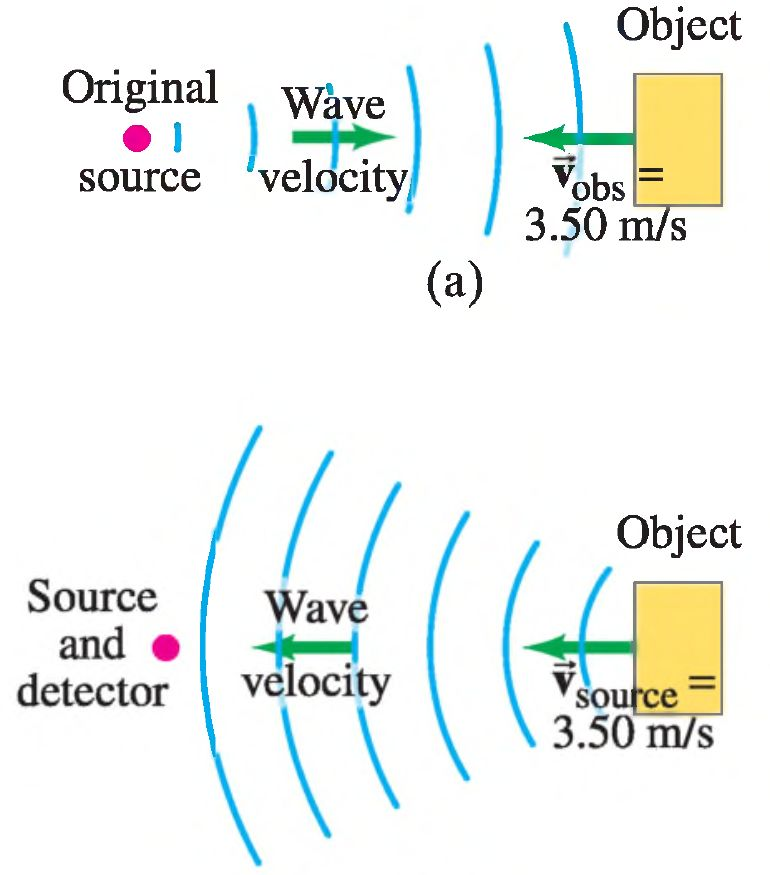
\includegraphics[height=2.in]{images4/doppler7.jpg}
\end{center}


  
   \column{2in}


The prequency emited by the "new" source is,

\begin{equation*}
f''=\frac{f'}{(1-\frac{v_{source}}{v_{snd}})}
\end{equation*}

   \end{columns}




  \end{frame}
%%%%%%%%%%%%%%%%%%%%%%%%%%%%%%%%%%%%%%%%%%%%%%%%%%%%%%%%%%%%%%%

\begin{frame}
\frametitle{Doppler Effect}

Example: 

\vspace{3mm}

   \begin{columns}[c]
   \column{2in}  % slides are 3in high by 5in wide
  \begin{center}
  \includegraphics[height=2.in]{images4/doppler7.jpg}
\end{center}


  
   \column{2in}


The frequency emitted by the "new" source is,

\begin{equation*}
f''=\frac{f'}{(1-\frac{v_{source}}{v_{snd}})}=5103~HZ
\end{equation*}

   \end{columns}




  \end{frame}


%%%%%%%%%%%%%%%%%%%%%%%%%%%%%%%%%%%%%%%%%%%%%%%%%%%%%%%%%%%%%%%

\begin{frame}
\frametitle{Doppler Effect}

We can summarize both effects in a single equation:

\begin{equation*}
f'= f\left(1+\frac{v_{obs}}{v_{snd}}\right)
\end{equation*}


\begin{equation*}
f'=\frac{f}{(1-\frac{v_{source}}{v_{snd}})}
\end{equation*}

\begin{equation}
f'= \frac{f}{(1-\frac{v_{source}}{v_{snd}})}\left(1+\frac{v_{obs}}{v_{snd}}\right)
\end{equation}


  \end{frame}


%%%%%%%%%%%%%%%%%%%%%%%%%%%%%%%%%%%%%%%%%%%%%%%%%%%%%%%%%%%%%%%

\begin{frame}
\frametitle{Doppler Effect}

Then, the frequency perceived by an observer when observer and source approach each other is,

\begin{equation}
f'=f \frac{v_{snd}+v_{obs}}{v_{snd}-v_{source}}
\end{equation}

\pause

And the frequency perceived  by an observer when observer and source move apart is,

\begin{equation}
f'=f \frac{v_{snd}-v_{obs}}{v_{snd}+v_{source}}
\end{equation}


  \end{frame}

%%%%%%%%%%%%%%%%%%%%%%%%%%%%%%%%%%%%%%%%%%%%%%%%%%%%%%%%%%%%%%%

\begin{frame}
\frametitle{Doppler Effect}

We can summarize all cases in a single equation:

\begin{equation}
f'=f \frac{v_{snd}\mp  v_{obs}}{v_{snd}\mp v_{source}}
\end{equation}

\pause

The upper signs in numerator and denominator apply if
source and/or observer move toward each other; the lower signs apply if they are
moving apart.

  \end{frame}

%%%%%%%%%%%%%%%%%%%%%%%%%%%%%%%%%%%%%%%%%%%%%%%%%%%%%%%%%%%%%%%

\begin{frame}
\frametitle{Doppler Effect}

Application:
\pause

\vspace{3mm}


The incident wave and the reflected wave in the last example interfere with one another and beats are produced.
\pause

\begin{itemize}
\item measuring the beats frequency, we can obtain the value of the moving object.
\pause
\item  For example, ultrasonic waves
reflected from red blood cells can be used to determine the velocity of blood flow.
\pause
\item the technique can be used to detect the movement of the chest of a
young fetus and to monitor its heartbeat.
\end{itemize}


  \end{frame}

%%%%%%%%%%%%%%%%%%%%%%%%%%%%%%%%%%%%%%%%%%%%%%%%%%%%%%%%%%%%%%%

\begin{frame}
\frametitle{Doppler Effect}

What happens if the source travels at a velocity equal or higher the sound velocity?

\pause


  \begin{center}
  \includegraphics[height=1.2in]{images4/shock_wave.jpg}
\end{center}






  \end{frame}


%%%%%%%%%%%%%%%%%%%%%%%%%%%%%%%%%%%%%%%%%%%%%%%%%%%%%%%%%%%%%%%

\begin{frame}
\frametitle{Shock Waves}

\begin{itemize}
\item When $v_{obj}<v_{snd}$ the pitch changes as we have seen $\rightarrow$ Doppler effect (b).
\pause
\item When  $v_{obj}=v_{snd}$, the crest of the wave fronts overlap, creating a big crest or barrier called the "Sound Barrier" (c).
\pause
\item When $v_{obj}>v_{snd}$,the source has broken the sond barrier so it  is  “outrunning” the waves it produces. The crests of numerous wave fronts are overlapped producing a shock wave (d). 
\end{itemize}

\pause

\vspace{3mm}

A very clear explanation: \url{https://www.youtube.com/watch?v=If-yK7sQE8Q}  


  \end{frame}


%%%%%%%%%%%%%%%%%%%%%%%%%%%%%%%%%%%%%%%%%%%%%%%%%%%%%%%%%%%%%%%

\begin{frame}
\frametitle{Questions}

\begin{itemize}
\item Two tuning forks oscillate with the same amplitude, but one
has twice the frequency. Which (if either) produces the more
intense sound?
\pause
\item How will the air temperature in a room affect the pitch of
organ pipes?
\pause
\item Is there a Doppler shift if the source and observer move in
the same direction, with the same velocity? Explain.
\end{itemize}

  \end{frame}


%%%%%%%%%%%%%%%%%%%%%%%%%%%%%%%%%%%%%%%%%%%%%%%%%%%%%%%%%%%%%%%

\begin{frame}
\frametitle{Questions}

Consider the two waves shown in the figure. Each wave can
be thought of as a superposition of two sound waves with
slightly different frequencies. In which of
the waves, (a) or (b), are the two component frequencies
farther apart? Explain.

  \begin{center}
  \includegraphics[height=1.5in]{images4/Q_ondas.jpg}
\end{center}


  \end{frame}


%%%%%%%%%%%%%%%%%%%%%%%%%%%%%%%%%%%%%%%%%%%%%%%%%%%%%%%%%%%%%%%

\begin{frame}
\frametitle{Questions}

The figure shows various positions of a child on a swing
moving toward a person on the ground who is blowing a
whistle. At which position, A through E, will the child hear
the highest frequency for the sound of the whistle? Explain
your reasoning.

  \begin{center}
  \includegraphics[height=1.5in]{images4/Q_ondas2.jpg}
\end{center}


  \end{frame}






%%%%%%%%%%%%%%%%%%%%%%%%%%%%%%%%%%%%%%%%%%%%%%%%%%%%%%%%%%%%%%%
 \end{document}
%%%%%%%%%%%%%%%%%%%%%%%%%%%%%%%%%%%%%%%%%%%%%%%%%%%%%%%%%%%%%%%